\documentclass[10pt,twoside]{report}

\usepackage[utf8]{inputenc}

\usepackage[dvipsnames]{xcolor}

\usepackage{graphicx}
\graphicspath{ {images/} }

\usepackage[a4paper,width=150mm,top=25mm,bottom=25mm,bindingoffset=6mm]{geometry}

\usepackage{fancyhdr}
\pagestyle{fancy}

\usepackage{soul}
\newcommand{\hlc}[2][yellow]{ {\sethlcolor{#1} \hl{#2}} }

\usepackage[numbers]{natbib}
\usepackage{color}

\usepackage{amsmath}
\usepackage{amsfonts}

\usepackage[ruled]{algorithm2e}
\usepackage{multicol}

\usepackage{tikz}
\usetikzlibrary{shapes.geometric, arrows}

\usepackage{etoolbox}
\apptocmd{\sloppy}{\hbadness 10000\relax}{}{}

\usepackage{caption}
\usepackage{subcaption}

\newcommand{\ys}[1]{{\color{red} \bf[YS: #1 ]}}

\title{
    {Dynamic Resource Allocation for Multi-Camera Systems}\\\vspace{1cm}
    {
\includegraphics[width=0.5\textwidth]{UvA-logo}}
}
\author{Eugenio Bargiacchi}
\date{\today}

\begin{document}

\maketitle

%\chapter*{Abstract}
%\chapter*{Dedication}
%\chapter*{Declaration}
%\chapter*{Acknowledgements}

\tableofcontents

\chapter{Introduction}\label{ref:intro}
\section{Active Perception}

The field of Active Perception focuses on efficiently employing sensors to gather data. This
decisional task is important in numerous real-world applications because of a number of factors:

\begin{itemize}
\item Limits in sensor number and capabilities. Ideally, we want to be able to obtain the maximum
performance possible from limited resources.
\item Energy, bandwidth and communication constraints. Not only these resources have a direct cost for
usage, but in many applications there are hard limits on how much a system is allowed to consume.
Again, we want to squeeze out as much performance is possible within our limits.
\item Storage constraints. It is important to reduce the amount of non-informative data that is gathered
by the sensors. Not everything is equally important. Being able to decide whether to gather data or
not helps in the long run maintaining reasonable sized data logs requiring less storage space and
easing possible future data searches.
\end{itemize}

In Active Perception there is no control over the environment; instead the task requires to affect
the way the available sensors collect data. This can mean actively directing sensors towards
environment areas that need to be observed, or by simply selecting the most informative subset
of data gathered by multiple sensors. All data gathered is then used in real time to further improve
the collection strategy, by automatically determining missing information that still needs to be
gathered.

Some of the great challenges faced by Active Perception systems are the following:

\begin{description}
\item[Knowledge Representation] The system managing the sensors needs to be able to correctly
maintain a representation of its knowledge, and how to gather more. This can get quite expensive
computationally when the size of the environment is non-trivial.
\item[Reward Measure] While knowledge representation is a problem in itself, the system also needs
to be able to tell which knowledge is actually important, and what measure of uncertainty it should
try to minimize. A popular target function is entropy; at the same time entropy estimation is a very
complex topic of research, and it has also been demonstrated that it is always subject to bias
\cite{cit:badentropy}.
\item[Action Selection] When multiple sensors are available the number of possible ways in which the
agent can observe the environment explodes exponentially, which usually requires some way to
approximate optimal action selection.
\item[Non-Myopicity] We argue that an optimal Active Perception solution needs to be able to take into
account the information that the system will be able to obtain in the future. This requires the
ability to forecast possible outcomes from the observation process in order to determine optimal
sequences of actions over continued periods of time.
\end{description}

All these problems make Active Perception systems very hard to scale effectively; at the same time,
real-world data gathering systems become bigger by the day. These challenges are what motivated this
thesis work.

\section{Application}

The applications of Active Perception cover essentially every possible use of sensors ever. It can
be used on physical detectors, like robotics, CCTV and surveillance, military reconnaissance. Or it
can be used to control data collection in virtual environments, such as social networks or online
retailer websites. In order to test our approaches, in this work we are going to consider the field
of multi-camera systems.

With the advent of cheap hardware, these last few years have brought an incredible widespread
adoption of multi-camera systems. These systems can be used for surveillance, real-time tracking and
many other purposes. Deployment expenses of such systems have progressively decreased with the
advent of digital multiplexing, the Internet and new manufacturing techniques. At the same time the
cost for operating the cameras and storing/analyzing the incredible amount of data they provide has
been increasing ever since, also due to their increasing numbers.

Although automatic mechanisms that try to record only useful footage do already exist the cameras
have still the need to be turned on at all times. An example of this are motion detectors. A motion
triggered camera would write its data to disk only when motion appeared on the screen, even though
the camera would still be on when nothing was happening in front of it, to keep the motion detector
on.

In addition to the "always on" problem, new video processing techniques can now be applied to
captured footage, such as face recognition and person tracking, which require non-trivial amount of
computation and bandwidth to be run together with the cameras themselves. This incurs in significant
energy and hardware costs, since they have to be applied to all cameras. Communicating all camera
data and perform remote computations can be even \textit{more} expensive.

Hard constraints on such resources make this field a great target for Active Perception. By
selecting at any one time a subset of cameras to use for detection, we reduce at the same time
energy costs, bandwidth and processing power, while at the same time trying to obtain the maximum
amount of information from the system.

A possible real-world application of multi-camera systems are Closed-Circuit Television (CCTV)
systems. More and more municipalities and private businesses are adopting them in order to improve
public safety and decrease crimes\cite{cit:cctv}. Though once widespread diffusion of this
technology was impaired by low image quality and a limited ability to record the camera view
requiring dedicated employees monitoring the video stream constantly, these limits have since been
overcome by new technology advances. At the same time, they can incur in significant energy and
communication costs \cite{cit:cctvenergy}.

\section{Research Questions}

Active Perception is an active field of research, and so many approaches to the problem have been
experimented with. In particular, this work tries to give an answer to the following questions,
which to our knowledge have not been answered yet:

\begin{itemize}
\item To what extent is a non-myopic solution necessary in order to achieve an optimal solution
within the Active Perception problem?
\item What are the trade-offs for using Monte Carlo approximations in Active Perception?
\end{itemize}

\section{Approach}

We are going to approach Active Perception by leveraging a powerful and flexible decision-theoretic
tool, called Partially Observable Markov Decision Process (POMDP) \cite{cit:pomdp}. We introduce
this powerful framework in Section \ref{ref:background}. POMDPs allow to model the interactions
between a decision making entity, called agent, and a partially observable, stochastic environment.
In this framework, the agent's objective is to maximize reward collection according to a predefined
reward function.

The main reason why we use POMDPs is that they easily allow for the computation of non-myopic
strategies for using the sensors. In fact, POMDPs are specifically structured as to allow this type
of planning. This means that the system will try to gather information in order to improve not only
its current knowledge of the environment, but also its future one. While myopic strategies can
sometimes be good approximations, we argue that to achieve optimality non-myopicity is required, as
shown in Chapter \ref{ref:experiments}.

In POMDPs, the agent tracks is current status via a \textit{belief}, which is a probability
distribution over the possible states of the underlying world. This belief is used to compute
possible outcomes for actions undertaken by the system, and to predict future rewards. This belief
is updated depending on the observation that the system receives from the sensors, taking into
account possible ambiguity (perceptual aliasing) that could result from imperfect knowledge.

Finally, POMDPs are a widely explored topic in the decision theoretic literature, with known
properties and already available solution methods, which allows us to stand on shoulders of giants.
We discuss on POMDPs solution methods in Chapter \ref{ref:background}.

One of the active topics of research in decision theory regards the efficient computation of POMDP
policies. When dealing with non-trivial models, the time needed to compute an optimal policy and the
space needed to store it increase exponentially with the complexity of the problem \cite{cit:pomdp}.
This has led to the development of methods that allow for approximate solutions.

In particular, our approach is based on online planning. This type of approach is based on
determining an optimal course of action applicable only to the situation that is currently faced by
the agent. This is in contrast with offline planning, where the whole problem is tackled at once
before deployment and the resulting policy stored for future usage. This usually requires a
significant amount of time in advance, and computation of the policy must be performed every time
the underlying model changes. The advantage of offline planning is that it requires virtually no
computing power when the final policy has to be applied by the agent, but at the same time the size
of problems that are currently possible to tackle in this way remain small.

On the other hand, online approaches can handle problems orders of magnitude bigger, at the expense
of having to compute the policy on the fly, requiring ultimately more processing power, but stretched
over time. At the same time, it is easier to experiment with different models, as there is no
pre-computation required. An example of the power of online methods are Monte Carlo methods, which
have demonstrated incredible performances in the Go board game \cite{cit:mcts}.

POMDPs in particular have been approached in an online way by approximating beliefs about the world
using particles, and using Monte-Carlo simulation to provide an effective way of approximating the
optimal solution \cite{cit:pomcp}.

At the same time, the active sensing problem is inherently about reducing uncertainty about the
world, which translates into a reward scheme based on the knowledge of the agent, rather than the
state of the world. Such a class of problems, denominated $\rho$POMDP, has been examined in
\cite{cit:rpomdp}. In this work we modify the existing Monte-Carlo POMDP approach to be able to work
using belief-based goals. This will allow an easily deployable and testable method to work with
active sensing problems.


\section{Contributions}

In this work we consider the problem of tracking a person moving throughout an environment which is
covered by a multi-camera system. We try to devise a centralized, intelligent method to
automatically activate cameras by predicting the movement of the target within range of the cameras,
and reducing as much as possible the uncertainty of their positions with limited resources. The idea
is to select the cameras which will provide the maximum amount of information within the available
resource limits. In a real world setting, such limits are generally defined as computational costs,
energy requirements and communication costs.

The camera selection problem is defined on already deployed systems, where camera positions and
orientations are known, and not modifiable. The goal is to be able to select a subset $k$ of the $n$
total cameras deployed, so as to maximize our knowledge of the state of the world; this is
equivalent of minimizing the entropy of our knowledge. In our particular approach, we consider the
case of tracking a single target using multiple sensors.

In this work we are going to use passive sensors in the form of fixed cameras. These cameras can be
seen as passive sensors since they only collect video information in a limited, non-interactive way.
The idea is to actively utilize these sensors by using only a subset of them at any time, in order
to reduce at the same time computational, energy and communication costs. We reduce energy by using
less cameras at any one time, and we can reduce computational and communication costs by reducing
the amount of data that needs to be processed concurrently.





\subsection{Chapter Overview}
Throughout Chapter \ref{ref:background} we introduce the background theory and models that support
our approach, and define the terms we use within this work. In Chapter \ref{ref:solutions} we
introduce the already existing techniques that led to our particular approach on the problem. In
Chapter \ref{ref:approach} we discuss the unique problems that we faced in this work, and our
proposed solutions. In Chapter \ref{ref:experiments} we show our experiments and results. Finally,
in Chapter \ref{ref:conclusion} we discuss our results and offer our insights.



\chapter{Background}\label{ref:background}

\section{Markov Decision Process}\label{ref:mdp}

The world is complicated. In order to be able to take decisions, a computer system needs to
understand how it works, and how it responds to actions. In order to do this, we want to wrap all the
complexity of the world into a mathematical framework to allow us to reason in a structured way. The
\textit{Markov Decision Process} (MDP), named after Andrey Markov, was developed for this task.

This framework is a simpler version of POMDPs, which we introduce later in Section \ref{ref:pomdp}.
It is used to model problems where the whole environment is visible at any moment by the agent, and
without fault. In practice, it is not able to handle partial observability, but it is still useful
since it introduces elements which we use later anyway. Its advantage over competing approaches is
its ability to easily produce non-myopic strategies, which do not act greedily on the short term,
but aim to maximize a goal over the long term.

In this work we assume that there is no learning to be done; any problem we model is known in
advance fully by the decision making entity. This entity can thus \textit{plan} its strategy in
advance, rather than learn it. This strategy is called a \textit{policy}.

The way we are going to create the framework is to split our world into two separate components: the
\textit{agent} and the \textit{environment}. The former represents our computer system and its
decision making abilities, while the second represents everything else.

An MDP can be defined formally as a tuple

\[ MDP = <S,A,T,R,\gamma> \]

The elements of the tuple are called state space, action space, transition function, reward function
and discount factor. We introduce these terms in the following Sections.

\subsection{Agent}

The agent is at the core of the decision process. It has a goal: to affect the environment so that
some form of "goodness" within it is achieved. The agent does not need to be part of the
environment, or be physically present within it; it is an abstract decision making entity. The only
thing the agent needs is a way to act upon the environment, so as to steer the way it changes
over time.

%In essence, the agent represents everything that we are able to control in an \textit{absolute} way
%within the world we have to work with. Unfortunately, this is not much. To make a simple example, in
%the case of a robot most often the physical body of the robot is part of the environment, rather
%than the agent. The agent, or brain, of the robot then acts so that the physical body moves,
%hopefully as predicted. But since the body can be subject to failure and precise movements and
%sensors are required to check whether a motion completed successfully, we regard it as environment.

In the MDP framework this connection is achieved through \textit{actions}. Each action has a
specific effect on the environment, and the agent tries to choose at any moment the most correct
one.

\subsection{Environment}

The environment represents all that is not the agent. Unfortunately the real world is usually much
too complicated to be constrained into a mathematical framework, so some descriptive approximations
can be used instead. Generally, the environment is described at a level of abstraction that allows
to predict effects with reasonable accuracy for the task at hand, without the need to specify
needless details which would only impede the decision making process. Just as a person does not
consider interactions on a molecular level when making coffee, we want to do the same for our
description of our environment.

In this way, we want to be able to describe our environment in terms of its possible configurations.
Each configuration, denoted \textit{state}, represents a unique arrangement of the world at any one
time. For example, in chess, the environment can be completely described by the positions of all
pieces on the game board. The full set of states is denoted \textit{state space}, and is usually
referred to as $S$. This is the first element of the MDP tuple.

\[ S = \{s_0, s_1, s_2, ..., s_{|S|}\} \]

Note that we assume that all sets presented in this thesis work to be finite, unless where
specifically noted.

In order to describe how the environment is allowed to change over time, we can define
cause-effect links between states. This is effectively equivalent to a state machine.

%Just as in a state-machine, we can now start to reason in which ways the
%environment is allowed to change, and what we should do to pick the path that mostly suits our
%goals. These links need not be deterministic: they can, and will very often be, stochastic. This
%stochasticity can be used to represent a real stochasticity of the world underlying our abstract
%environment, or can be used to abstract away details that we know exist but are unwilling to model
%to reduce overall complexity. All in all, these two options are often much the same. In a dice roll,
%we could decide to model all physical forces acting on the dice, or just model the result as a
%stochastic number taken at random.

In the environment, transitions between a state and another state are discrete and instantaneous.
Each transition happens within a single \textit{timestep}, which represents the atomic unit of time
within the environment. Note that timesteps can be abstract, as they do not have to be directly
linked with time. Rather, a timestep is associated with environment changes that are significant to
the decision process, and so tie again to the concept of a state-machine. Whether those changes
happen in hours of real time or in seconds - or whether different changes occur with different
durations - does not influence the framework.

%A very important property of our environment, however, is that it is not allowed to contain any
%external decision-making entities. This is because such entities are themselves able to influence
%the evolution of the environment over time in ways our agent cannot predict, and modeling them
%though a state-machine framework is next to impossible. A whole branch of decision theory is
%dedicated to the study of such systems: multi-agent problems are by far more complex than
%single-agent ones.
%
%In our particular problem, prediction of people movement within a location, each person can be seen
%as an external entity which decides autonomously where it wants to move. Trying to model each and
%every person fully is a hopeless endeavor. At the same time, in the context of walking from a point
%A to a point B, people can be fairly predictable. Thankfully, evolution made us realize a long time
%ago that the fastest way to travel between two points is a straight line, and that can help in
%predicting where a person is going to go. Even though the path of each single person will be hard to
%predict with perfect accuracy, we can predict possible alternatives stochastically with a decent
%degree of accuracy, and that allows us to ignore the problem of multiple independent autonomous
%entities affecting the world simultaneously.

\subsection{State}

As we said above, our environment is described through states, which all together form the
\textit{state space} of the problem. Each state is unique, meaning that it represents a unique
circumstance of the environment, different in some particular way from all others. At the same time,
a state is a unique representation of the environment that ignores all that is not relevant to the
decision making progress. In a chess game, it does not matter whether at the time of playing it's
raining, but only the position of the pieces on the board.

%There are multiple ways of defining the states of the environment. One way is to enumerate them all.
%In this case, each state is in some sense independent from all others, and must be specified
%uniquely and added to the state space. This is called an \textit{extrinsic} definition of the state
%space. On the other hand, it is possible to define a number of features to define all states. In this
%way, a feature is a particular property of the environment that can take on a certain number of
%values. Following, a state is defined by the values all features are taking at any one time, and the
%whole state-space results from the product of all features. To keep with the chess analogy, one
%could describe every possible position by a combination of the position of every single piece - a
%feature. Such description of the state space is called \textit{intrinsic}.

An extremely important property that each state needs to have is called the \textit{Markov}
property. This property requires that the evolution of the environment depends only on the
information encoded in its current state, and nothing else. This can also be seen as saying that the
environment has no memory, since keeping track of previous states has no use for its future
evolution. The Markov property is required in order to allow the agent to reason only about the
current state, without the need to know its history.

While it can happen that a particular environment can evolve in a time-sensitive manner, it can be
easily shown that all such environments can be modeled in a Markovian way by simply adding more
features into the state-space definition \cite{cit:boutilier}.

\subsection{Action}

An action is a way in which the agent can influence the environment. Although in the problem that is
specifically considered in this work the agent has no control over the evolution of the environment
in the more general MDP framework actions can also be used to alter the way the environment can
evolve over time. In our problem we use a POMDP, which directly links actions to observations, where
the agent can actively collect information about the environment. Actions are thus relevant even
when the environment cannot be directly changed. We refer to Section \ref{ref:obsspace} for discussion
about this topic.

Actions can represent some actual action the agent is allowed to take, such as activating a motor,
or can express a more abstract function, such as a robot walking forward. These abstract actions can
then be performed by simpler subroutines which perform all the required intermediate steps to
complete the full action. The only requirement for the definition of an action is that its
consequences on the environment are understood.

The full set of actions available to the agent is called the \textit{action space}, or otherwise
referred to as $A$. This is the second element of the MDP tuple. It is usually assumed that all
actions are available to the agent at any timestep.

\[ A = \{ a_0, a_1, a_2, ..., a_{|A|} \} \]

\subsection{Transition Function}

In an MDP, the evolution dynamics of the environment are encoded in a function, called
\textit{transition function}. This function allows to specify the interrelations between each state
and each action, and the consequences of actions in terms of environment progression over time.

In particular the transition function is a function

\[ T: S\times A \times S \rightarrow [0,1] \]

that specifies the probability for any transition in the environment, depending on the actions that
the agent can take. In other words, it specifies the probability that by applying a particular
action in a particular state, we end up into a second state. Using this function, the agent can
determine the best way to reach a particular state from any other state. Another way to see this
function is to look at it as representing a conditional probability function:

\[ T(s, a, s') = Pr(s' | s, a) \]

Where $Pr(s'|s,a)$ is the probability of the environment transitioning to $s'$ from $s$ when the
agent performs action $a$. By using this notation, we can additionally show mathematically what the
Markov property is about. This property holds when

\[ Pr(s_{t+1} | s_{0}, a_{0}, s_{1}, a_{1}, ..., s_{t}, a_{t} ) = Pr(s_{t+1} | s_t, a_t ) \hspace{1cm} \forall s \in S \]

\subsection{Reward Function}

We use a similar function, called the \textit{reward} function, to encode the goals that we wish the
agent to achieve. This function is once again defined upon states and actions, but can take values
within the real domain:

\[ R: S\times A\times S \rightarrow \mathbb{R} \]
\[ R(s, a, s') \in \mathbb{R} \]

Encoding goals as numbers can initially be quite strange if someone is not used to it. What this
function represents is the level of appeal that a particular situation or outcome represents to the
agent. For example, we can specify whether a particular state of the environment is preferable over
another, and as such transitions that lead to the former are represented with a higher number in
the reward function. Or, we could prefer rewarding the agent for a particular effort, setting the
reward function to high values when a particular action is tried in a particular state. On the other
hand, negative terms can be used to inflict penalties over particular events that we do not want to
happen.

In these terms, all possible achievements and penalties have a weight and can be compared to each
other, in order to allow the agent to determine which goal to pursue depending on circumstances. The
usage of numbers is necessary in order for this weighting to take place at all.

Note that the reward function specifies a reward for each single transition the agent encounters,
independently from the current timestep. It occurs often that most of the transitions have no
particular reward, but the agent still needs to consider all of them when computing its policy.

After defining the reward function, one can start to imagine how the MDP framework operates. The
agent has access to actions, and it knows how these actions affect the environment via the
transition function. Using this function it can determine the best sequence of actions to select in
order to steer the environment towards a particular state. Finally, the state to reach is determined
by weighting pros and cons of any specific trajectory within the environment, and all intermediate
rewards the agent could pick up along the way.

\subsection{Discount and Horizon}

As we mentioned before, an MDP is a tool that takes into account future rewards in order to compute
the best possible policy. The agent does in fact try to maximize its \textit{expected return} within
an \textit{episode}: the expected sum of all rewards obtained within a single try at the task. We
can define it as a simple summation:

\[ \mathbb{E}[\text{return}] = \mathbb{E} \left [ \sum_{t=0}^h R(s_t, a_t, s_{t+1}) \right ] \]

An important fact is that the optimal policy is very dependent on the exact amount of time that the
agent thinks it's going to act within the environment. This time is called \textit{horizon}, and is
represented by $h$ in the above equation.

An horizon of 1 timestep generates what is generally known as a \textit{greedy policy}. Such a
policy acts in a locally optimal way, hoping that in doing so it will act in an optimal way
globally. As the horizon increases the final policy takes into account more and more possible
outcomes, becoming more complex but, depending on the task, more performant overall. On the opposite
side of a single step horizon, we have an \textit{infinite horizon}. Policies computed for infinite
horizons would be infinitely complex, but what happens in general is that policies tend to converge
as the horizon grows, so it is possible to have a very simple policy for an infinite horizon.

Infinite horizons have a disadvantage though. While in finite horizons the agent has an incentive as
to act optimally, in order to obtain the maximum possible reward within its alloted time, in an
infinite horizon there is no such urgency. Reward obtaining actions can be postponed indefinitely,
since in the limit the reward the agent will be able to obtain will remain the same (infinite).

A different way of presenting the concept of horizon is with the concept of \textit{discounting}.
Discounting makes rewards less valuable the further away in time they get collected. A simple
real-world example are banks interest rates: they lend money in the present, and to compensate for
that, they ask in return more money in the future. This is precisely because obtaining something now
is more valuable than obtaining it in the future.

An agent thus tries to maximize the \textit{expected discounted return}. All gained rewards are
decreased geometrically by a discount factor $\gamma \in [0,1]$:

\[ \mathbb{E}[\text{discounted return}] = \mathbb{E} \left [ \sum_{t=0}^h \gamma^t R(s_t,
a_t, s_{t+1}) \right ] \]

In this way, rewards that are far in the future become essentially meaningless, forcing the agent to
consider the present as more important of the far future. In essence, we are forcing the discounted
return to converge to a finite quantity. When $\gamma$ is 0 we have a single-step problem, where the
agent wants to maximize its currently available reward using a greedy policy.  When $\gamma$ is 1 we
have again the situation where there is no incentive for an agent to act, since it will still be
able to act in the future. $\gamma$ is the fifth and final element of the MDP tuple.

\subsection{Policy}

At this point we have introduced all elements that compose the MDP. Here we talk about the solution
itself, how it looks like and what it represents, while postponing the discussion about solving
algorithms for Section \ref{ref:solutions} onward.

A solution for an MDP is called a \textit{policy}. This policy specifies a sequence of actions to
be taken by the agent, depending on the states the agent will face while acting in the model. In
general we are interested in what is called the \textit{optimal policy}, which is the one whose
actions maximize the expected (discounted) return: it behaves better than all other policies on
average. Policies can be stochastic, so that in a given state there may be multiple action options
from where one is randomly picked up.

The policy's decisions take into account the chosen horizon for the problem. Thus, the policy's
decisions are dependent on the number of timesteps that the agent has still left to act. We can
define a policy $\pi$ as a function, that given an horizon, a state and action returns the
probability of the action being chosen:

\[ \pi : H \times S \times A \rightarrow [0,1] \]
\[ \pi(h, s, a) \in [0,1] \]

We can also define it as a function, taking a state and an horizon, returning a distribution over
action, which one can sample:

\[ a \sim \pi(h, s) \]

A useful property of the optimal policy is that is composed recursively. An optimal policy for
horizon $h$ only defines a single action to be taken per state. Once that action has been performed,
the agent can safely adopt the optimal policy for horizon $h-1$ from its resulting next state. This
means that any optimal policy for a particular horizon also contains implicitly all optimal policies
for all lower horizons.

\subsection{Value Function}

Since the environment, as encoded in the transition function, is stochastic, the agent cannot
predict with full accuracy which states it will experience during an episode, nor how much reward a
certain sequence of actions will be able to accumulate. What it can do instead is to compute the
expected return that will be obtained, as in the average cumulative reward that the agent would
collect if it was allowed to retry the same sequence of actions from the same state many, many
times. This expected return is of course computed with respect to a certain policy, since as we said
the reward obtained depends on which actions the agent performs.

The expected return depends on the state $s$ the environment is in where the agent needs to act.
Thus it is also called the \textit{value} of state $s$ with respect to, or under, some particular
policy $\pi$. This value of course depends also on how many steps the agent has left to take.
Formally then we can define the value of a state as:

\[ V^\pi_{s\:h} = \mathbb{E}^\pi_h \left [\text{discounted return} \mid s_0 = s \right ] \]
\[ = \mathbb{E} \left [\sum_{t=0}^{h} \gamma^t R(s_{t}, a_t, s_{t+1}) \right ]
    \hspace{0.5cm}\text{where }s_0 = s \text{ and }a_t \sim \pi(h-t, s_t) \]

This value is very important because it lets us compare and evaluate policies. A better policy does
in fact have a higher value or equal value for every possible state than an inferior policy.

An even more important property of value functions was discovered by Richard Bellman. It is a way of
representing a value function in terms of itself, recursively. The value of a state can thus be
defined as

\[ V^{\pi}_{s\:h} = \sum_a \pi(h, s, a) \sum_{s'} T(s, a, s') \left [ R(s, a, s') + \gamma
V^{\pi}_{s'\:h-1} \right ] \]

This is also known as the \textit{Bellman equation}. The value of a state can be thus computed as
the expected reward that the agent can obtain in the next timestep, plus a discounted total which
represents what is going to happen in the future. The fact that this equation is recursive is
immensely important and forms a base for many offline planning algorithms.

In general, when we are looking for a solution we are looking for a policy $\pi^*$that maximizes the value
of all states:

\[ V^{\pi^*}_h = \max_\pi V^{\pi}_h \]

\subsection{Q-function}

A function that is closely tied with the value function is the \textit{Q-function}. The Q-function
also contains values with respect to a policy and a state, but they also depends on an action. The
Q-function represents the value a state would have if we performed such an action, and followed the
specified policy from there after. In short:

\[ Q^{\pi}_{h}(s,a) = \sum_{s'} T(s, a, s') \left [ R(s, a, s') + \gamma
V^{\pi}_{s'\:h-1} \right ] \]

The Q-function also has an optimal version, $Q^*$, which depends, of course, on $V^*$. Extracting an
optimal policy from $Q^*$ is extremely easy, as it is possible to simply perform a maximization on
the actions over the Q-function, and the best action is automatically found.

\[ a^* = \arg\max_a Q^*_h(s,a) \hspace{.5cm}\forall s \in S\]

Many solution methods rely on the direct approximation of the optimal Q-function in order to find
the optimal policy. One of the beauties of this approach is the optimal policy can computed via a
single-step maximization of the Q-function. This is because the Q-function already encodes
internally the expectations over future rewards, and in this way allows us to perform a simple
greedy maximization to obtain a non-myopic solution.

\section{Partially Observable MDP}\label{ref:pomdp}

The framework we have described in Section \ref{ref:mdp} is used in order to model environments
where the agent has full access to state information during the full course of each an any episodes.
In an MDP, in fact, the agent is always able to reason simply in terms of the current state, and
take current decisions based on that information.

In the real world, however, most always an agent does not have access to the true underlying state
of the world. Instead what often happens is that the agent has access to imperfect sensors, which
rely incomplete information useful to understand in which state the environment is currently in. The
agent then needs to take into account the probability that the environment is in a state versus another
before deciding how to act.

Thus we extend the MDP framework into a \textit{Partially Observable Markov Decision Process}
(POMDP). In a POMDP all terms that we have defined previously are still used and taken into account,
but we are going to add on to these definitions a couple more.

A POMDP can be defined as a tuple $<S,A,T,R,\Omega,O,\gamma>$. We now define $\Omega$ and $O$.

\subsection{Observation}\label{ref:obsspace}

In a POMDP the agent does not have access to the current state of the environment. The state is
still there, and the environment is always in a particular state at any timestep, but the agent has
no direct way to know which one it is. The agent instead receives, at each timestep, an
\textit{observation}, which depends on the action that the agent performed and on the new state that
has been reached.

All observations are, as are states and actions, grouped in a set, $\Omega$, where usually $|\Omega| <
|S|$.

\[ \Omega = \{ o_0, o_1, o_2, ..., o_{|\Omega|} \} \]

\subsection{Observation Function}

The framework models the way the agent is able to receive information from observation as an
additional function added on top of the MDP framework. This function is called the
\textit{observation function}. It is a function

\[ O : S' \times A \times O \rightarrow [0,1] \]

so it relays the probability of receiving a certain observation upon reaching a given state $s'$
after taking action $a$.

\[ O(s', a, o) = Pr(o | s', a) \]

Note that the state is the one of \textit{arrival}, not the one where the action is performed.

\subsection{History and Belief}

The observation function does not allow the agent to disambiguate between states, or the problem
would convert directly to an MDP. Instead, what happens is called \textit{perceptual aliasing}: each
obtained observation is compatible with a subset of $S$. The agent must reason about which of the
possible underlying states of the environment are compatible with the observation obtained in order
to plan its moves.

Unfortunately, this implies that the agent is now unable to reason about the present. While the
environment states maintain their Markov property, the agent cannot observe them. Instead it needs
to store internally its whole history of actions and observations in order to keep track of which
states are possible at any point in an episode. This long list of actions and observations is called
\textit{history}.

An alternative way of maintaining the history is keeping a \textit{belief} over the current state of
the environment. Such a belief is simply a probability vector in $|S|$ dimensions, where each
element denotes the probability that the environment is in a particular state. Such a representation
becomes a very powerful abstraction that allows the computation of values with respect to beliefs.

At each new timestep, the agent's belief needs to be updated with the new knowledge gained by the
agent. The belief can be updated with the following formula:

\[ b'(s') = \frac{O(s', a, o)\sum_{s\in S}T(s,a,s')b(s)}{Pr(o|a,b)} \]

The denominator can be treated as a normalizing factor that makes $b'$ correctly sum up to 1, since
it is a probability vector.

\subsection{Belief MDP}

The belief allows for a reinterpretation of the POMDP framework. The belief can in fact be used in
lieu of a state, since it is possible to compute new transition and reward functions that depend on
beliefs rather than states. This transforms automatically the POMDP into an MDP, where the
belief is now the state of the agent.

We can show how this can be done using $\tau$ as the new transition function and $\rho$ as the new
reward function:

\[ \tau(b,a,b') = \sum_{o\in \Omega} Pr(b' | b, a, o) \sum_{s\in S} O(s,a,o) b(s) \]

Where

\[Pr(b' | b, a, o) = \left\{
  \begin{array}{lr}
    1 \hspace{.6cm}\text{if the belief update with arguments $b,a,o$ returns $b'$}\\
    0 \hspace{.6cm}\text{otherwise}
  \end{array}
\right.
\]

Similarly:

\[ \rho(b,a) = \sum_{s\in S} R(s,a) b(s) \]

Although this transformation allows us to forget the partial observability, we have now introduced a
new problem: a continuous state space. Although continuous MDPs are very hard to solve generally,
the belief MDP can be approached due to a property of its value function.

\subsection{Value Function}

In the MDP framework a value function needs to store a value for each possible state in the
environment. Since the number of states in the belief MDP is infinite, in theory a full value
function would be impossible to store, and the same would hold for any policy. However, in the case
of a belief MDP we can leverage a particular property of the value function that lets us avoid this
problem.

The value function of a POMDP is a function dependent on beliefs. Thus, the value function is
defined on a simplex space of $|S|-1$ dimensions. The property that makes POMDPs tractable is
that their value function is \textit{piecewise linear and convex} (PLC). In addition, the number of
polytopes of which it is composed has a finite bound at any horizon - exponential in the number of
possible observations.

These properties bound the number of optimal values that actually need to be stored, as only one
value for each linear polytope needs to be stored, making possible to solve a POMDP exactly. For a
more in-depth analysis of POMDP properties refer to \cite{cit:pomdp}.

\subsection{Policy}

A policy in a finite-horizon MDP is a set of sequences of actions that need to be taken, where each
such sequence is associated with a single state. This allows the agent to act no matter what it is
its starting state.

This is similar in a POMDP, with the difference that a different sequence of actions needs to be
stored for each linear polytope of the value function, instead that for each unique belief. The
optimal policy maintains the recursive property that we have defined previously for MDPs, where any
strategy for a particular horizon $h$ and belief $b$ is composed by a particular action plus the
optimal policy for horizon $h-1$.

%\section{Generative Model}% START FROM HERE
%
%What we have described up until now are models which assume that you have a lot of explicit
%knowledge about the problem you want to solve. This is because you need to know perfectly the
%transition function, observation function and reward function. Having this kind of intimate
%knowledge of a problem is, unfortunately, relatively rare.
%
%Thankfully, in order to apply Monte-Carlo techniques there is no need to have this level of detail
%in the description of a problem. Instead it is possible to work solely on a generative model which
%the agent can sample from in order to reproduce the behavior of the world, but is at the same time a
%black box with respect to its inner workings. Samples drawn from a generative model are
%indistinguishable from those sampled from a full-fledged model.
%
%Generative models are useful as one can gather real world data from an unknown stochastic process
%and use it to feed a Monte-Carlo planner, without the need to accurately study the process and
%determine exact probabilities and rewards for the transition and reward functions. It can also
%happen that computationally, a generative model is faster to run than a model which requires
%maintaining huge internal tables to store the transition and reward functions.
%
%In both cases, it is important to keep in mind that not all components of an MDP need to be directly
%available in order to be able to compute a good policy.

\section{$\rho$POMDP}

As we have already mentioned, in a POMDP the reward is defined in terms of the belief, as a linear
combination of the basic MDP reward function:

\[ \rho(b,a) = \sum_{s\in S} R(s,a) b(s) \]

However, in many cases, such as ours, this definition is limiting and cannot be used. If the reward
function is truly dependent on the information the agent has on the current state of the world,
rather than on the underlying state of the world itself, the MDP reward function becomes useless,
and as such our definition of $\rho$. In the case of surveillance, the agent actions should maximize
the knowledge that the agent has of the world, independently of which state the world is currently
in.

In this case, the $\rho$ function is defined independently, and not tied to states anymore.
Unfortunately, this means giving up on the PLC properties of the value function, which
were the only ways in which we were able to solve a POMDP in the first place. While it has
been proved in \cite{cit:rpomdp} that as long as the newly defined $\rho$ function is PLC then the
value function will be PLC as well, functions such as entropy are not PLC in the first place. We
discuss how we overcame this problem in Section \ref{ref:approach}.

\section{Planning vs Reinforcement Learning}\label{ref:solutions}

While often the possible states, actions and observations of a particular environment are easy to
define, it does not always happen that the transition, observation and reward functions are known in
advance.

When they are known, the solving process is called \textit{planning}, and consists in efficiently
looking through all possible transitions the agent could experience, and finding the best path
through them in order to maximize the return.

On the other hand, when they are not known, \textit{reinforcement learning} is used. In this case the
focus is on gathering knowledge about the environment while \textit{at the same time} exploiting that
knowledge to obtain the maximum return. Reinforcement learning methods can range from approximating
the unknown functions from experience and then planning, to approximating the optimal value function
of the model and using it to obtain a policy, or even directly approximating the optimal policy.

In this work we assume we are either given a model, or a model is learned in advance, and that this
model is used as a base for planning.

\section{Offline vs Online}

An optimal policy can be applied at virtually no computational cost with the knowledge that the
behavior is constantly optimal. Computing such a solution in advance and using it later is called
\textit{offline planning}. The main disadvantage of offline planning is its very heavy upfront cost:
it needs to store all possible policies to be applied to any reachable belief at any horizon. This
is expensive not only in terms of space, but even more on computation, since any non-trivial POMDP
has an exponential explosion in the number of possible histories that an agent can experience and
each one of them has to be considered in order to evaluate the final policy \cite{cit:pomdp}. In
addition, any small change in the original model requires a full recomputation of the optimal
policy, which limits the amount of tuning that can be feasibly done on the model.

Offline planning methods generally leverage the Bellman equation and the recursive nature of the
value function; they plan in reverse temporal order, from the last steps the agent will take to the
first ones. This is because a policy for a certain horizon $h$ is always composed by a set of
actions to apply in certain beliefs which then leads to a policy for horizon of $h-1$. Thus, the
final policy needed is computed incrementally. All possible state, actions and observations are
considered, so as to provide the correct action in every possible situation.

In order to avoid the computational cost of offline methods, a new venue of approach was invented
called \textit{online planning}. In online planning the agent continuously plans for its current
belief, and nothing else. This requires constant computations, but at the same time makes possible
to tackle problems orders of magnitude bigger than what is possible with offline planning, and allow
for flexibility in updating the model, since there is no need to recompute a complete solution. In
addition, many online planning methods are \textit{any time}: this means that they can run for
whatever time is available, and they are always able to provide some sort of solution. The more time
is available, the more refined the solution will be. This is in contrast with offline methods, that
need to run to completion or otherwise nothing is gained.

In online planning computations go forward in time. From the current state/belief of the agent
possible futures are expanded in a tree of possibilities and rewards. In the end, the best action
for the current state is picked, the environment is advanced one step, and the process repeats
again.

In this work we chose to use an online approach, given the flexibility and power provided over
offline techniques, and because one of our goals was to scale to real-world scenarios, which are
generally intractable with offline approaches. An additional advantage which we will explore later
is that online planners are able to deal with non-PWLC value functions, which is a challenge when
using negative entropy as a reward function.

\section{Monte Carlo Algorithms}

At the time of writing, one of the most promising ways of planning online is by using \textit{Monte
Carlo algorithms}. Monte Carlo algorithms are a class of randomized algorithms which use random
processes in order to compute their output. The output will be correct within a certain probability,
which trades off with their speed and their deterministic running time.

In the MDP/POMDP frameworks Monte Carlo algorithms only need results from samples of the
environment; as in, transition and reward results sampled from the model's distribution using
particular state-action pairs as inputs. Such a model is also called a \textit{generative model}. A
generative model $G$ fed with state $s$ and action $a$ would return a new state $s'$ and reward $r$
respecting the model probabilities:

\[ s', r \sim G(s, a) \]

An advantage of using such a model is that it many cases it is possible to obtain samples without
having the whole transition function for the model in an explicit form. The samples obtained can
then be used to approximate average returns, which in turns can be used to obtain an optimal policy.

\section{Monte Carlo Tree Search}

The most widely known algorithm using Monte Carlo techniques is called \textit{Monte Carlo Tree
Search} (MCTS) \cite{cit:mcts}. This algorithm is an MDP online planner which has received high
praise for its contributions in the development of highly performant board game AIs.

MCTS was originally devised as a method to approach the board game Go. The algorithm runs Monte
Carlo simulations from the current state of the agent, which is the input, and progressively builds
a tree of outcomes.

\begin{algorithm}
\begin{multicols}{2}
    \caption{Monte Carlo Tree Search}
    \SetKwFunction{mcts}{MCTS}
    \SetKwFunction{simulate}{Simulate}
    \SetKwFunction{rollout}{Rollout}

    \SetKwProg{main}{Algorithm}{}{}
    \main{\mcts{s}}{
        \KwData{State s}
\nl     \While{enough time is available}{
\nl         \simulate{\O, s, 0}\;
        }
\nl     \KwRet most valued action in tree root\;
    }

    \setcounter{AlgoLine}{0}
    \SetKwProg{myproc}{Procedure}{}{}
    \myproc{\rollout{s, d}}{
        \KwData{State s, Depth d}
\nl     r = 0\;
\nl     discount = 1\;
\nl     \While{$d <$ horizon}{
\nl         ($s', r'$) $\sim$ G($s$, random action)\;
\nl         r = r + discount * $r'$\;
\nl         discount = discount * $\gamma$\;
\nl         $s$ = $s'$\;
        }
\nl     \KwRet r\;
    }

    \setcounter{AlgoLine}{0}
    \SetKwProg{simul}{Procedure}{}{}
    \simul{\simulate{h, s, d}}{
        \KwData{History h, State s, Depth d}
\nl     select action $a$\;
\nl     ($s', r$) $\sim$ G($s,a$)\;
\nl     \If{$d < $ horizon}{
\nl         \eIf{T($h,a,s'$) is not \O}{
\nl             futureRew = \simulate{$(h,a,s'), s', d+1$}\;
            }{
\nl             initialize T($h,a,s'$)\;
\nl             N($h,a$) = V($h,a$) = 0\;
\nl             futureRew = \rollout{s', d+1}\;
            }
\nl         r = r + $\gamma$ * futureRew\;
            }
\nl     N($h,a$) = N($h,a$) + 1\;
\nl     V($h,a$) += $\frac{r-V(h,a)}{N(h,a)}$\;
\nl     \KwRet r\;
    }

\end{multicols}
\end{algorithm}

The MCTS tree of outcomes starts out as a single root. This root represents the current state of the
agent. From this root MCTS carries out as many sample episodes as possible. After each sample
episode, the MCTS tree is expanded, keeping track of all possible futures experienced by MCTS.

Each sample episode can be divided into two phases: in the first the algorithm descends the
known tree, while in the second the algorithm simulates outside it.

Descending the tree is done recursively in a very simple fashion. Starting from the root node $s$, the
algorithm selects an action $a$, and uses both to produce a reward $r$ and a next state $s'$. The
action is selected probabilistically, with more promising actions selected more often.  The root
children are then searched for a node representing the sequence $(a,s')$. If one is found, the
algorithm descends one level in the tree, and repeats the action selection and sampling process,
this time using the last $s'$ as its $s$.  This repeats until the algorithm is unable to descend
further into the tree.

Once the bottom of the tree is reached, the algorithm adds a single child node to the reached leaf.
The node represents the $(a,s')$ from the last sample. Once this is done, MCTS enters its
second phase.

During the second phase the algorithm continues to simulate the episode, but it does not use the
tree anymore. Actions are selected using a \textit{rollout policy}, which is generally uniformly
random. This continues until a terminal state or the selected horizon is reached. This concludes the
sample episode.

Once a sample episode ends, all the reward collected during both phases is backpropagated up to the
tree root. This is used to update the values of all the actions taken during the first phase of the
algorithm.

At this point, a new sample episode is started from the root of the tree. This process is repeated
until there is time left.

A nice property of MCTS is that it is guaranteed to converge to the optimal policy as long as the
most promising actions are given a higher probability of being chosen than the others. This is
because in the long run the value averages will converge to the values of the actions taken most
often.  In addition, since it builds a tree, part of the work done can be reused on the next time
step. Once a move is tried in the real world, the tree root can be moved to the new state perceived,
while the rest of the tree is discarded.

\section{Upper Confidence Bounds for Trees}

A technique which has recently gained popularity to exactly determine which actions should be chosen
within the tree and which ratio should be used between promising actions and the rest is called
\textit{Upper Confidence Bounds for Trees} (UCT) \cite{cit:uct}. UCT tries to empirically derive a
variance estimate from the data, sorting actions by their upper bounds on value.

The upper bound estimate is composed of two parts: the currently estimated value of the action $v$,
and the estimated UCT variance. Thus the value that UCT assigns at a given action $a$ is:

\[ UCT(a) = v + c*\sqrt{\frac{\log{N}}{n}} \]

Where $N$ is the number of times the node in the tree currently being considered has been visited,
and $n$ is the number of times action $a$ has already been tried from the node. $c$ is a constant
which is dependent on the problem, which defines the amplitude of the variance, which needs to be in
tune with the magnitude of the rewards of the MDP. This number is generally tuned manually, and is
around the maximum return that can be obtained by the agent.

Actions are then selected greedily with respect to the UCT value.

\section[]{Partially Observable Monte-Carlo Planning%
\sectionmark{POMCP}}
\sectionmark{POMCP}

\textit{Partially Observable Monte-Carlo Planning}(POMCP) \cite{cit:pomcp} is one of the
state-of-the-art online solvers available today. This algorithm incorporates the advantages of MCTS
while adding support for belief states and observations.

The trouble of naively applying MCTS to a belief MDP extracted from a POMDP is its necessity to
sample directly from state to state. While this can be a cheap operation in MDPs, requiring
samples from relatively simple distributions, computing a new belief given a previous belief and
observation in a POMDP, called \textit{belief update}, can be a very expensive operation. Recall that a belief
update can be performed using the following formula:

\[ b'(s') = \frac{O(s', a, o)\sum_{s\in S}T(s,a,s')b(s)}{Pr(o|a,b)} \]

For a full belief, this requires $O(|S|^2)$ operations, which for POMDPs with a large state space
can result in an extremely expensive operation. Since MCTS requires a very high number of samples in
order to provide useful answers, each sample needs to be performed in as little time as possible.

POMCP solves this problem by representing beliefs as particle vectors containing a certain amount of
state particles. Such a \textit{particle belief} can be created by repeatedly sampling a belief, and
gathering all samples in a vector - not a set.

\begin{algorithm}
    \caption{Partially Observable Monte-Carlo Planning}
\begin{multicols}{2}
    \SetKwFunction{pomcp}{POMCP}
    \SetKwFunction{simulate}{Simulate}
    \SetKwFunction{rollout}{Rollout}

    \SetKwProg{main}{Algorithm}{}{}
    \main{\pomcp{b}}{
        \KwData{Belief b}
\nl     \While{enough time is available}{
\nl         s $\sim$ b\;
\nl         \simulate{\O, s, 0}\;
        }
\nl     \KwRet most valued action in tree root\;
    }

    \setcounter{AlgoLine}{0}
    \SetKwProg{myproc}{Procedure}{}{}
    \myproc{\rollout{s, d}}{
        \KwData{State s, Depth d}
\nl     r = 0\;
\nl     discount = 1\;
\nl     \While{$d <$ horizon}{
\nl         (s', r') $\sim$ G(s, random action)\;
\nl         r = r + discount * r'\;
\nl         discount = discount * $\gamma$\;
\nl         s = s'\;
        }
\nl     \KwRet r\;
    }

    \setcounter{AlgoLine}{0}
    \SetKwProg{simul}{Procedure}{}{}
    \simul{\simulate{h, s, d}}{
        \KwData{History h, State s, Depth d}
\nl     select action $a$ with UCT\;
\nl     ($s', o, r$) $\sim$ G($s,a$)\;
\nl     \If{$d < $ horizon}{
\nl         \eIf{T($h,a,o$) is not \O}{
\nl             futureRew = \simulate{$(h,a,o), s', d+1$}\;
            }{
\nl             initialize T($h,a,o$)\;
\nl             N($h,a$) = V($h,a$) = 0\;
\nl             futureRew = \rollout{s', d+1}\;
            }
\nl         r = r + $\gamma$ * futureRew\;
            }
\nl     B(h) = B(h) $\bigcup \;\{ s' \}$\;
\nl     N($h,a$) = N($h,a$) + 1\;
\nl     V($h,a$) += $\frac{r-V(h,a)}{N(h,a)}$\;
\nl     \KwRet r\;
    }

\end{multicols}
\end{algorithm}

POMCP starts its execution in the root of the tree, which represents the current particle
belief of the agent. POMCP, as MCTS, is again composed of two phases: tree descent and outside tree
simulation. The procedures for both are very similar to the MCTS originals.

Starting from the root, POMCP samples a single state $s$ from the root's particle belief. Then,
using UCT, it selects a state $a$, and uses both to sample a new state $s'$, a reward $r$ and an
observation $o$. The root children are then searched for a node representing the sequence $(a,o)$. If
one is found, the algorithm descends one level into the tree. While descending, POMCP appends $s'$
to the particle belief of the selected child node. Then, it repeats the action selection and
sampling process using $s'$ as its $s$. This repeats until the algorithm is unable to descend
further into the tree.

The adding of particles to lower level particle beliefs is the way POMCP updates beliefs, without
the $O(|S|^2)$ complexity.

Once the bottom of the tree is reached, the algorithm adds a single child node to the reached leaf.
The node represents the $(a,o)$ from the last sample. It also adds to the new node's particle belief
its first particle, the final $s'$. Once this is done, POMCP enters its second phase.

During the second phase the algorithm continues to simulate the episode, but it does not use the
tree anymore. Actions are selected using a \textit{rollout policy}, and observations sampled are
completely discarded. This continues until a terminal state or the selected horizon is reached. This
concludes the sample episode.

Once a sample episode ends, all the reward collected during both phases is backpropagated up to the
tree root. This is used to update the values of all the actions taken during the first phase of the
algorithm.

At this point, a new sample episode is started from the root of the tree. This process is repeated
until there is time left.


\chapter{Approach}\label{ref:approach}
\section{Myopicity of Active Perception}

As we have already said, POMDPs can be used naturally to compute non-myopic policies to solve a
particular task. However, in order to justify the usage of POMDPs, we have to demonstrate that the
Active Perception task requires the usage of non-myopic solutions in the first place.  This is
because not all problems necessarily require non-myopic solutions.

\ys{reword this statement, we dont have to justify usage of POMDPs, its should be more along the lines of, we believe pomdp provides a natural framework for modelling this kind of task ( which we have already conveyed to user in introduction and background) }

We propose two different POMDP models of Active Perception problems. For one of the models we will
prove that a non-myopic solution is required in order to obtain an optimal solution. For the second
we will prove that a non-myopic solution is not required. The results we show are for both max of
belief and negative entropy reward functions.

\ys{Again, rather write this para as we have tried myopic and non-myopic approaches in different settings. In some settings, myopic policy proved to be as optimal as nonmyopic, where as in some settings non myopic policy has a clear advantage over myopic. We discuss the nature of this phenomenon in detail later.}
\ys{why are models still in approach?}

While we were not able to demonstrate a general way to show whether any particular problem will need
non-myopicity in the solution, the fact that Active Perception tasks exist which require
non-myopicity is sufficient to motivate our choice of POMDPs in this work.

\subsection{Non-Myopic World}

Let's consider a world where the agent is tasked with tracking a single person that is walking. The
person can, at any moment, be in one of a series of rooms, and can transition between them. In each
room there is a camera which can observe the room itself and nothing else. If the agent activates
the camera situated in a room the person just entered there is a $0.8$ probability that the agent will
obtain a ``found'' observation, and a $0.2$ probability that it will obtain a ``null'' observation.
On the other hand, if the agent activates any other camera, it will obtain a ``null'' observation
with $0.8$ probability and a ``found'' observation with $0.2$ probability. Each time a camera is
activated, the person will move to another accessible room. The agent's goal is to guess correctly
where the person has moved for two times in a row, knowing only that at the start the person could
be in any room.

We will now create an instance of the problem we have just finished describing. Let's now suppose
that in our world there are 6 rooms, and we know that the person will transition from one to another
with the following probabilities:

\begin{center}
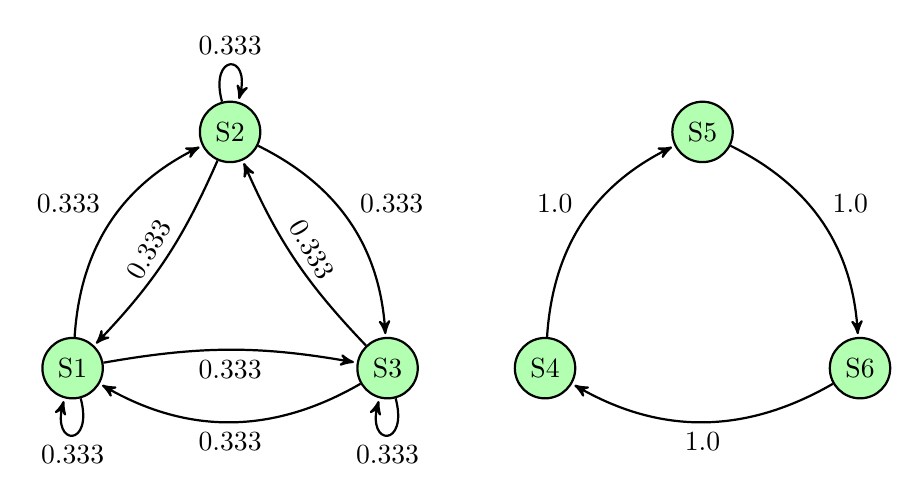
\begin{tikzpicture}[->,>=stealth',shorten >=1pt,auto,node distance=4cm,thick,main node/.style={circle,draw,font=\Large\bfseries}]
\tikzstyle{state} = [circle, draw=black, fill=green!30]
\tikzstyle{arrow} = [thick,->,>=stealth]

\node (s1) at (0,0) [state] {S1};
\node (s2) at (2,3) [state] {S2};
\node (s3) at (4,0) [state] {S3};
\node (s4) at (6,0) [state] {S4};
\node (s5) at (8,3) [state] {S5};
\node (s6) at (10,0) [state] {S6};

\path
    (s1) edge [loop below] node {0.333} (s1)
         edge [bend left] node {0.333} (s2)
         edge [bend left=10] node[below] {0.333} (s3)
    (s2) edge [loop above] node {0.333} (s2)
         edge [bend left=10] node[above,rotate=60] {0.333} (s1)
         edge [bend left] node {0.333} (s3)
    (s3) edge [loop below] node {0.333} (s3)
         edge [bend left=10] node[above,rotate=-60] {0.333} (s2)
         edge [bend left] node {0.333} (s1)
    (s4) edge [bend left] node {1.0} (s5)
    (s5) edge [bend left] node {1.0} (s6)
    (s6) edge [bend left] node {1.0} (s4);

\end{tikzpicture}
\end{center}

As we said, at first the agent does not know where the person is at all. The myopic expected return
for the first step only is:

\[ E[\text{return}| a_1 ] = \sum_{o\in \Omega} p(o | b, a_1) \cdot \rho(b') \]

Where $b'$ is the result of the belief update of $b$ with $o$ and $a_1$. The non-myopic expected return over
both steps is:

\[ E[\text{return}| a_1, a_2] = \sum_{o \in \Omega} p(o | b, a_1) \left ( \rho(b') + \sum_{o' \in
\Omega} p(o'| b', a_2) \cdot \rho(b'') \right ) \]

Where $b''$ updates from $b'$, $o'$ and $a_2$. It is easy to show that, both for max of belief and
negative entropy as $\rho$, all actions in the presented problem have the same myopic one-step
expected return from a uniform belief. This is done by simply computing the previously described
summatory over every term and performing the appropriate belief updates.

However, expected non-myopic returns are not the same for all choices of $a_1$ and $a_2$. For
example selecting $a_1 = S1$ always results in a certain expected return $v$, independently from
$a_2$. On the other hand, if $a_1 = S4$, all expected returns are greater than $v$ for all but one
choice of $a_2$. In other words, selecting $a_1 = S1$ leads necessarily to a lower two-step expected
return, since the agent can select $a_2$ to only pick the best cases.

Selecting $a_1$ to avoid the worst cases can only be done when there is a way to distinguish between
two different $a_1$.  Since myopic expected returns are the same for all $a_1$, this is impossible
to do with a myopic solution.

Note that the problem considered can be extended into uncountably many models where the same
properties apply. This could be done for example by adding a certain number of rooms that the person
needs to go through before ending up in the model presented, and so on. Thus a non-myopic solution
is required for uncountably many Active Perception tasks.

\ys{I feel this whole section about models and consequences should be in experiements and the consequence or explanation about what is happening should be in discussion or experiments.}

\subsection{Myopic World}

A different instance of the previous problem is one where there are only 4 rooms, and the person
will transition from state to state with the following probabilities:

\begin{center}
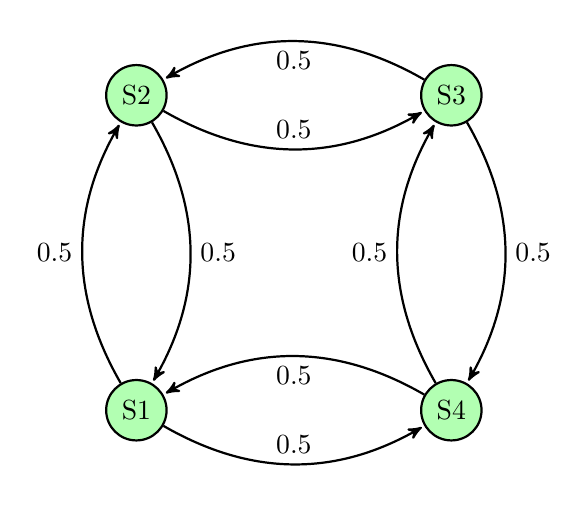
\begin{tikzpicture}[->,>=stealth',shorten >=1pt,auto,node distance=4cm,thick,main node/.style={circle,draw,font=\Large\bfseries}]
\tikzstyle{state} = [circle, draw=black, fill=green!30]
\tikzstyle{arrow} = [thick,->,>=stealth]

\node (s1) at (0,0) [state] {S1};
\node (s2) at (0,4) [state] {S2};
\node (s3) at (4,4) [state] {S3};
\node (s4) at (4,0) [state] {S4};

\path
    (s1) edge [bend right] node {0.5} (s4)
         edge [bend left] node {0.5} (s2)
    (s2) edge [bend left] node {0.5} (s1)
         edge [bend right] node {0.5} (s3)
    (s3) edge [bend right] node {0.5} (s2)
         edge [bend left] node {0.5} (s4)
    (s4) edge [bend left] node {0.5} (s3)
         edge [bend right] node {0.5} (s1);

\end{tikzpicture}
\end{center}

Once again, we can compute both myopic and non-myopic expected returns. This time, no matter the
choice of actions, there is no particular incentive for an agent to select a pair over another. If
$\rho$ is negative entropy, certain pair of actions have a higher expected return than others. But
for each $a_1$ there is a $a_2$ which obtains the maximum expected return possible.

Thus, non-myopic in this particular model has no particular advantage over a more simple myopic
solution. Once again this problem can be extended into uncountably infinite examples of Active
Perception tasks.

\section{$\rho$-POMCP}

In this Section we present a modification of the algorithm POMCP which is able to deal with a
belief-based reward function in POMDPs. An important fact to note that this algorithm is able to
deal with any $\rho$-POMDP, and not only with Active Perception tasks. For example, this algorithm
can be applied to problems where the agent can influence the state of the world, and also (with
minor modifications to reintroduce state dependent rewards) when the reward function is both
dependent on states and belief.

\ys{you should explain here why POMCP cannot be applied to $\rho$ POMDP or any POMDP with belief dependent reward directly.}


\subsection{Non-PWLC Value Function}

Negative entropy is not a PWLC function. This means that the value function of a $\rho$-POMDP which
uses it as reward function will not be PWLC too \cite{cit:rpomdp}. This is a problem for offline
planning since usual solving techniques rely on the PWLC property in order to detect beliefs where
the currently computed optimal policy is not actually optimal. Once such a belief point is
discovered (called \textit{witness point}), the optimal policy is updated to be optimal in that
belief too.

This problem is solved in our approach since online planning does not suffer from that problem. This
is because online planning directly approximates rewards for the possible futures of any given
situation, without the need to solve a POMDP completely for any possible beliefs. Thus, witness
points do not need to be discovered, and we can ignore the PWLC property.


\ys{this is a potential source of confusion. $\rho$ POMDP has a PWLC value function and thus can be solved offline. This leads back to discussion we had about what is $\rho$POMDP and what is not. I know that the paper quotes that any POMPD with belief dependent reward is $\rho$ POMDP. However, the main distinctive property about $\rho$ POMDP is not that they were the first to define the reward in terms of $\rho$, but they were the first to take a $\rho$ defined reward and find a way to approximate it with PWLC function. This para sounds like it is not possible to solve $\rho$POMDP offline, and that is why we need your method, which is not true. You should use term 'POMDP with belief-dependent reward'}

\subsection{Reward Estimation}

The main challenge when applying POMCP to a $\rho$-POMDP is that the algorithm can only extract
reward information from a generative model. This cannot be done for a belief-dependent reward
function, since the belief is an abstraction created by the agent, which does not actually exist in
the environment.  Thus, a generative model is unable to sample from a belief-dependent reward
function.

\ys{Previous comments apply here too. $\rho$POMDP has a way of defining a belief dependent reward in terms of state.(which is what POMDP IR also does). However, in online planning, for any method that is not sampling based, it should be possible to compute future rewards directly from belief. In our case, since POMCP is a sampling based algorithm, we have to find a way of keeping estimates of belief-based rewards depending on the samples. Again this para sounds like POMCP cannot be applied to $\rho$POMDP, which is not true.}

To avoid this, we estimate the immediate reward for a specific action-observation transition by
using maximum-likelihood estimates of the belief extracted from the particle beliefs POMCP
generates. However, since particle beliefs are updated constantly, computing a direct estimate of
every belief reached during each sample episode would excessively hamper performance. We solved this
problem differently for estimating max of belief rewards and negative entropy rewards.

For estimation of max of belief, $\rho$-POMCP simply keeps track of the number of particles in each
particle belief, the number of particles for each type of particle and which type of particle is the
most common. At each particle insertion the number of particles for that type is compared against
the number of the old most common particle. Whichever is higher becomes the new most common
particle, and the new max of belief is computed as the ratio between the most common particle count
and the total number of particles in the belief.

\ys{is there a better way to differentiate particles and 'type of particle'. I can understand what you are trying to say, but the word particle causes too much confusion here.}

\begin{algorithm}[H]
    \caption{Max of Belief Reward Estimation}
    \SetKwFunction{update}{Update Estimate}

    \SetKwProg{main}{Algorithm}{}{}
    \main{\update}{
        \KwData{Particle Belief b, Particle s}
\nl     N(s) = N(s) + 1\;
\nl     \If{N(s) $>$ N(max\_s)}{
\nl         max\_s = s\;
        }
\nl     $\rho(b)$ = $\frac{N(max\_s)}{N(b)}$\;
    }
\end{algorithm}

For estimation of entropy, the situation is not quite so straightforward. Entropy estimation from
discrete samples is bound to be biased, and there is no way to remove this bias completely
\cite{cit:badentropy}. On the other hand, techniques to decrease bias are computationally heavy and
rely on usage of additional complex distributions to account for bias \cite{cit:entropyfixes}.
Since $\rho$-POMCP needed to be as fast as possible, we decided to try a more direct approach in the
hope that any inaccuracies would not hamper significantly the search process.

Negative entropy is computed as a summation of terms, one for each type of particle:

\[ -H(b) = \sum_s p(s) \log p(s) \]
\[ -H(b) \approx \sum_s \frac{n_s}{N} \log \frac{n_s}{N} \]

$\rho$-POMCP stores internally both the latest negative entropy estimate $-H(b)$, and each of the
separate terms that compose it. At each new particle insertion in a particle belief, we simply
remove from our previous full estimate the relevant term for the particle state, recompute the term
and add it again. This approach is not mathematically correct as, in theory, all terms would need to
be updated at each insertion. This is because each entropy term depends on the probability of such
term, which in turn depends on the total number of particles in the belief, which has just been
increased by one. In essence, we are overestimating negative entropy. Again, we would have bias
anyway no matter the strategy we used.

\begin{algorithm}[H]
    \caption{Negative Entropy Reward Estimation}
    \SetKwFunction{update}{Update Estimate}

    \SetKwProg{main}{Algorithm}{}{}
    \main{\update}{
        \KwData{Particle Belief b, Particle Type s}
\nl     $\rho(b)$ = $\rho(b)$ - $\rho(s)$\;
\nl     N(s) = N(s) + 1\;
\nl     p = $\frac{N(s)}{N(b)}$\;
\nl     $\rho(s)$ = p $\cdot$ log(p)\;
\nl     $\rho(b)$ = $\rho(b)$ + $\rho(s)$\;
    }

\end{algorithm}

In practice, this bias turns out not to be a problem as long as each type of particle is added with
relative frequency, so as to keep all terms that compose the overall negative entropy ``fresh''.
Such an approach is in any case guaranteed to converge to the true entropy in the limit, when the
number of samples tends to infinite. This maintains the POMCP property that leads to an optimal
solution in the limit.

\ys{explanation of computation of entropy estimates can be structure this way. 1.) We follow the following procudeure to compute entropy estimates. 2). However, this procedure causes bias and other problems. 3) Earlier results show that bias is difficult to get rid of and other problems. 4) In practice, bias does not matter as long as we have a lot of samples. Right now these points seems a bit mixed with each other. }


\subsection{Value Backpropagation}

A second problem is dependent on how returns are approximated \ys{computed or approximated?} in POMCP. The value for a
belief-action pair $b,a$ \ys{isnt this just $Q(b,a)$} is computed as the sum of two different factors: the immediate reward
$\rho(b,a)$ plus a discounted term representing the expected return from then on.

\[ V(b,a) = \rho(b,a) + \gamma \cdot \sum_{o\in \Omega} O(o|b,a) V(b') \]

\ys{should be Q}

Recall that in a belief MDP the reward function is defined as:

\[ \rho(b,a) = \sum_{s\in S} R(s,a) b(s) \]

To approximate this value POMCP simply averages all results from $R(s,a)$ done using particles
extracted from the all beliefs and actions encountered during sample episodes.

\[ V(b,a) \approx \frac{\sum_{s \in S} n_s R(s,a)}{N} + \gamma \cdot \frac{\sum_{o\in \Omega} n_o f_o}{N} \]

Where $N$ is the number of times that action $a$ has been taken in belief $b$, $n_s$ the number of
times state $s$ has been sampled from $b$ when taking action $a$, $n_o$ is the number of times that
observation $o$ has been seen from $b$ and $a$ and $f_o$ is the average of all values backpropagated
from lower in the tree after observation $o$. In POMCP a backpropagated value is simply the
discounted sum of all sampled rewards down in the episode. As with MCTS, as long as the better
actions are chosen more often than the others, this procedure will converge to the true expected
return.

\ys{this parts needs to be written a bit more formally and using a conventional notation. ex: V(b,a) is Q(b,a). It is very difficult to understand what $f_{o}$ is ??}

However, in our case, the reward function is structured in the following way:

\[ \rho(b,a) = \sum_{o\in \Omega} O(o | b, a) \rho(b') \]

This is because both max of belief and negative entropy rewards can be only extracted from a belief,
and do not depend on actions. Thus, the value for a belief-action pair becomes:

\[ V(b,a) = \sum_{o\in \Omega} O(o | b,a) \rho(b') + \gamma\sum_{o\in\Omega} O(o|b,a) V(b') \]

The problem is that we estimate $\rho(b')$ directly, rather than by averaging samples. At the same
time, $V(b')$ depends on reward estimates of future beliefs, which again are estimated directly.
This means that whenever a new estimate for any given $\rho(b)$ is computed, the new value needs to
substitute the previous one all the way up the chain, and cannot be simply averaged in as it
happened in POMCP.

We solved this problem by keeping the average mechanism present in POMCP, with the difference that
we average together fake datapoints built specifically to replace previous estimates. For
example, suppose we have a particular estimate $r$ for $\rho(b, a)$.

\[ \rho(b,a) \approx r \]

We can decompose this into all our estimates for all beliefs reachable from $b$ and $a$:

\[ \rho(b,a) \approx \frac{\sum_{o\in\Omega} n_o r_o}{N} \]

Suppose now we experience $b$ and $a$ again, and obtain observation $\tilde{o}$. We update our new
reward estimate for the new belief into $r'_{\tilde{o}}$. If we averaged normally, we would get:

\[ \rho(b,a) \approx \frac{ n_{\tilde{o}} r_{\tilde{o}} + r'_{\tilde{o}} +
\sum_{o \neq \tilde{o} \in \Omega} n_o r_o}{N+1} \]

This is not what we want, however. Instead, suppose we average in $n_{\tilde{o}}(r'_{\tilde{o}} -
r_{\tilde{o}}) + r'_{\tilde{o}}$:

\[ \rho(b,a) \approx \frac{ n_{\tilde{o}} r_{\tilde{o}} + n_{\tilde{o}}(r'_{\tilde{o}} -
r_{\tilde{o}}) + r'_{\tilde{o}} +
\sum_{o \neq \tilde{o} \in \Omega} n_o r_o}{N+1} \]

\[ \rho(b,a) \approx \frac{ n_{\tilde{o}} r_{\tilde{o}} + n_{\tilde{o}}r'_{\tilde{o}} -
        n_{\tilde{o}} r_{\tilde{o}} + r'_{\tilde{o}} +
\sum_{o \neq \tilde{o} \in \Omega} n_o r_o}{N+1} \]

\[ \rho(b,a) \approx \frac{ ( n_{\tilde{o}}+1) r'_{\tilde{o}} +
\sum_{o \neq \tilde{o} \in \Omega} n_o r_o}{N+1} \]

Which is what we wanted. Similarly, we can create fake reward points to backpropagate in the tree so
that any $V(b)$ can be substituted with the more up-to-date $V'(b)$. The value backpropagated would be:

\[ N ( V'(b) - V(b) ) + V'(b) \]

\subsection{Max vs Mean}

The POMCP algorithm averages together all sampled rewards, and depends on UCT to let the tree
converge to the true optimum. This works since UTC samples the best actions infinitely more often in
the limit, which lets the final estimated value for it converge to the true value. However, this
procedure needs to sample many more times to make up for the fact that, at first, results for
suboptimal actions are averaged into estimates too.

POMCP inherits this behaviour from the original MCTS algorithm. However, in the original paper from
2006 a number of different approaches to merge together backpropagated values were tried
\cite{cit:mcts}. The authors decided to stick with using the mean operator to backup values since,
with the computational power available at the time, it gave better and more consistent results.
However, the authors also demonstrated that if enough samples are available, using a max operator
over actions actually improves performance.

We implemented both backup methods for $\rho$-POMCP in order to determine which one would perform
best under different conditions.

\subsection{Algorithm}

Here we describe the full $\rho$-POMCP algorithm in more detail.

\begin{algorithm}[H]
    \caption{$\rho$-Partially Observable Monte-Carlo Planning}
\begin{multicols}{2}
    \SetKwFunction{pomcp}{$\rho$-POMCP}
    \SetKwFunction{simulate}{Simulate}

    \SetKwProg{main}{Algorithm}{}{}
    \main{\pomcp{b}}{
        \KwData{Belief b}
\nl     \While{enough time is available}{
\nl         s $\sim$ b\;
\nl         \simulate{\O, s, 0}\;
        }
\nl     \KwRet $\arg\max_a V(a)$\;
    }

    \setcounter{AlgoLine}{0}
    \SetKwProg{simul}{Procedure}{}{}
    \simul{\simulate{h, s, d}}{
        \KwData{History h, State s, Depth d}
\nl     N($h$) = N($h$) + 1\;
\nl     select action $a$ with UCT\;
\nl     ($s', o$) $\sim$ G($s,a$)\;
\nl     \eIf{T($h,a,o$) is \O}{
\nl         initialize T($h,a,o$)\;
\nl         newNode = true\;
        }{
\nl         newNode = false\;
        }
\nl     B($h,a,o$) = B($h,a,o$) $\bigcup \;\{ s' \}$\;
\nl     \eIf{$d < $ horizon and newNode == false}{
\nl         r = \simulate{$(h,a,o), s', d+1$}\;
        }{
\nl         N($h,a,o$) = N($h,a,o$) + 1\;
\nl         r = $\rho(h,a,o)$\;
        }
\nl     N($h,a$) = N($h,a$) + 1\;
\nl     V($h,a$) = V($h,a$) + $\frac{r - V(h,a)}{N(h,a)}$\;
\nl     oldV = V($h$)\;
\nl     V($h$) = $\rho(h)$ + $\gamma \cdot \max_{a'} V(h,a')$\;
\nl     \KwRet N($h$) * ( V($h$) - oldV ) + V($h$);
    }
\end{multicols}
\end{algorithm}

$\rho$-POMCP starts off as POMCP, by simulating episodes from the root of the tree.

Starting from the root, $\rho$-POMCP samples a single state $s$ from the root's particle belief.
Then, using UCT, it selects a state $a$, and uses it with $s$ to sample a new state $s'$, a reward
$r$ and an observation $o$. The root child representing the sequence $(a,o)$ is selected, or if it
did not exist, it is created. The algorithm then updates the particle belief of the child before
deciding whether to continue to descend the tree. While descending, POMCP appends $s'$ to the
particle belief of the selected child node. Then, it repeats the action selection and sampling
process using $s'$ as its $s$. This repeats until the algorithm is unable to descend further into
the tree, at which point the future reward is approximated as simply the reward of the last
selected child's belief.

The algorithm then updates the value of all actions taken during the descent, while backpropagating
fake datapoints to update all old reward estimates up in the tree.

Notice that $\rho$-POMCP lacks a rollout procedure. This is because $\rho$-POMCP has no way to
approximate rewards when outside the tree, and so skips random policy rollouts altogether.

\section{Multi Person}

One of the main limiting factors for Monte-Carlo online methods is the branching factor of the
tackled problem. While MCTS, POMCP and $\rho$-POMCP can deal with incredibly large state and
observation spaces, they cannot deal easily with a problem that leads to a vast number of branches
to be explored. This is because each new branch significantly increases the number of sample
episodes that need to be performed in order to obtain an accurate estimate for the best action.

The main branching factor in the problem we are considering, which is multi-sensor systems, is the
number of targets to be tracked. This is because each target moves independently, and thus from a
given state there are many more possible states reachable. Thus, the branching factor for a problem
is exponential in the number of targets.

In order to avoid dealing with this problem, we setup a system where we run concurrently many
$\rho$-POMCP instances. Each solver computes an individual policy for a single target only and
receives individual observations. This allows each solver to work on a relatively small tree,
without exploding the number of branches. In addition, this allows to work with a variable number of
targets, since it possible to dynamically adjust the number of online planners running at any time,
depending on the number of targets present in the environment.

We then estimate the final action to be performed by merging the separate results of all the
solvers.  From each solver we then obtain a value estimate for each available action; the final
action is then the one that maximizes the sum of all values across solvers. In order to obtain
consistent evaluations of all root actions so that we can compare them between solvers, we disable
UCT for the first depth level in the tree, and instead sample equally from each action.


\chapter{Related Work}\label{ref:relwork}
\section{Active Perception}

The Active perception task has been approached in numerous ways.

% \cite{cit:relworkneuralnet} approach the Active Perception task using reinforcement learning through
% a neural network. The neural network has the task of recognizing a particular visual pattern, which
% is observed through a visual sensor, which can only read portions of the pattern at any single time.
% The neural network has the ability of moving the sensor in various ways, obtaining visualizations of
% the pattern from different point of views. Their approach requires training for every recognized
% pattern
%
% PROBLEM: It is RL, we do planning

% \cite{cit:relworkconvex} tackle the problem of selecting $k$ sensors out of a pool of $n$ sensors.
% They approximate the information function defined from the usage of any $k$ sensors with a convex
% function, that can be then solved efficiently with linear solvers. Once this is done, the found
% solution is checked for improvements by testing possible swaps with the sensors that were not selected.
%
% PROBLEM: In the end I don't really tackle multi-sensor here..

% \cite{cit:relworklagrange} tackle multi-sensor system management, considering dynamic programming
% and linear solvers in order to balance the trade-offs between gathering information and energy costs
% due to communication.
%
% PROBLEM: I don't really get the paper, it's way too complex..

\ys{add related work on entropy estimation. A little bit about work from paninski} 
\ys{add a little bit more about earlier solutions to dynamic sensor selection problem 
\begin{itemize}
\item Approximate dynamic programming for communication-constrained sensor network management. Do they use closed-loop polcies? Check for that, point that as difference, also you use UCT for planning that is another difference. 
\item Sensor selection via convex optimization. The same points as above.
\end{itemize}
}
\citet{cit:relworktanks} tracks the movement of multiple targets using a scan sensor. To keep track
of each target position they use weighted Monte-Carlo particles which are updated using a model of
the environment. Action selection tries to maximize the expected Rényi information divergence to
reduce entropy with respect to the posterior distribution of targets. They extend their approach to
non-myopic solutions by direct enumeration of all possible outcomes. A key difference is that we
track each target separately, thus reducing the complexity of the overall posterior distribution of
targets. In addition, our usage of POMDPs to model the environment allows computations of non-myopic
strategies in a much more natural way than direct enumeration. 

\citet{cit:relworkentropy} examine a localization problem using direction-of-arrival sensors. They
analyze the usage of an entropy-based heuristic to select a single sensor at a time step, and show
that on average the heuristic is able to select the sensor which maximizes the mutual information
between target location and sensor observation. Their approach does not approximate heuristic
calculations, requiring $O(S^2)$ time to evaluate a single sensor, which becomes prohibitive when
the space to observe is very large. We avoid this cost by using Monte Carlo simulations to
approximate entropy estimations.

\citet{cit:relworkspaan} use POMDPs to approach the multi-sensor system management problem, where
only a subset of $k$ sensors out of a pool of $n$ sensors can be selected. Their approach is based
on state-based reward functions, where the agent is rewarded for activating cameras with a target in
the field of view. Their approach focused on approximate offline planning for the model using
the SYMBOLIC PERSEUS algorithm, a variant of PERSEUS \cite{cit:perseus}. A crucial difference
is that our work does not rely on an offline planner, and thus does not have to recompute a solution
in case of a change, and can be more easily applied to much bigger models.

\citet{cit:relworksatsangi} use 

\section{Online POMDP Solvers}

One of the earliest explorations into online POMDP solvers has been been done by
\citet{cit:relworkonline1}, resulting in the Real-Time Belief Space Search (RTBSS) algorithm. This
algorithm creates a tree out of every possible result, and computes full belief updates and value
backups in order to determine the best actions at each step. In order to decrease computational
cost, a branch and bound strategy is employed to avoid exploring actions that have been proved not
useful. This strategy, however, can be used only by computing bounds offline, and then applying that
information to the leaves on the tree.

Other algorithms, such as BI-POMDP \cite{cit:relworkonlinebi} and AEMS \cite{cit:relworkonlineaems}
function similarly to the RTBSS algorithm, but rely on internal heuristics, rather than a branch and
bound strategy, to determine how to prune the tree to explore.

These algorithms differs importantly in that they try to solve the current belief perfectly. This
results in problems scaling when the number of possible actions and observations is high. By using
a Monte Carlo approach we avoid that problem by sampling, which allow our algorhtm to focus on
probable branches of the tree.

% An alternative to tree exploration approaches is the RTDP-BEL algorithm \cite{cit:relworkonlineq}.
% This algorithm learns progressively values for a discretized set of beliefs from direct interaction
% with the environment, using a Q-Learning type of approach.
%
% PROBLEM: RL

Our work in particular is based upon POMCP, an online solver that takes its strengths from
Monte-Carlo simulations \cite{cit:pomcp} which we discussed in Section \ref{ref:pomcp}. In
particular, POMCP follows the approach of Monte Carlo Tree Search, which progressively builds a tree
of outcomes by using a generative model to generate sample outcomes. This tree is then used to
approximate the values of all states. POMCP uses particle approximations of beliefs throughout this
tree, in order to avoid the expensive cost of computing belief updates at every action-observation
step. The difference with our approach is that POMCP cannot deal with belief dependent rewards, and
thus cannot evaluate policies which are tasked with increasing knowledge.

A good overview of existing POMDP online approaches can be found in \cite{cit:relworkonlineall}.

\section{Reward Estimation}

Our work employs reward estimation due to our


\chapter{Experiments}\label{ref:experiments}
\section{Myopic World}

\begin{figure}[h]
        \centering
        \begin{subfigure}[t]{0.3\textwidth}
                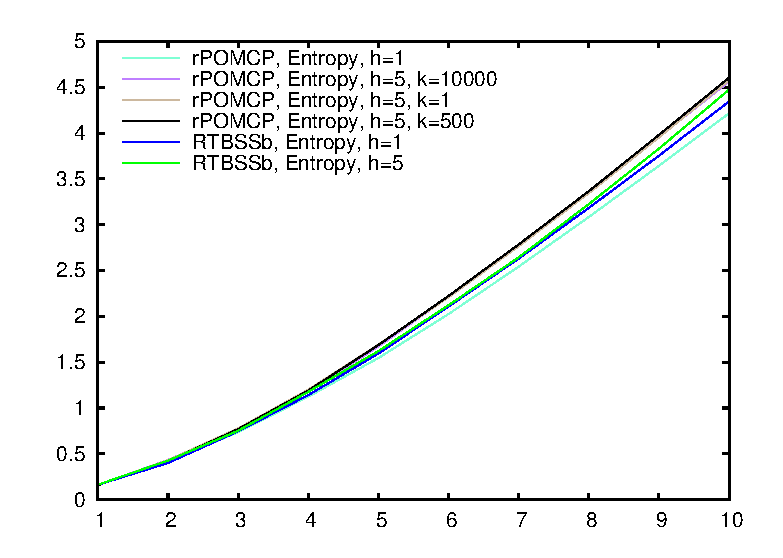
\includegraphics[width=\textwidth]{Images/MyoResults/1e4/E/output}
                \caption{Results in the Myopic World using 1e4 samples and entropy based reward
                function. RTBSS is not affected by this parameter.}
                \label{fig:m4e}
        \end{subfigure}%
        ~ %add desired spacing between images, e. g. ~, \quad, \qquad, \hfill etc.
          %(or a blank line to force the subfigure onto a new line)
        \begin{subfigure}[t]{0.3\textwidth}
                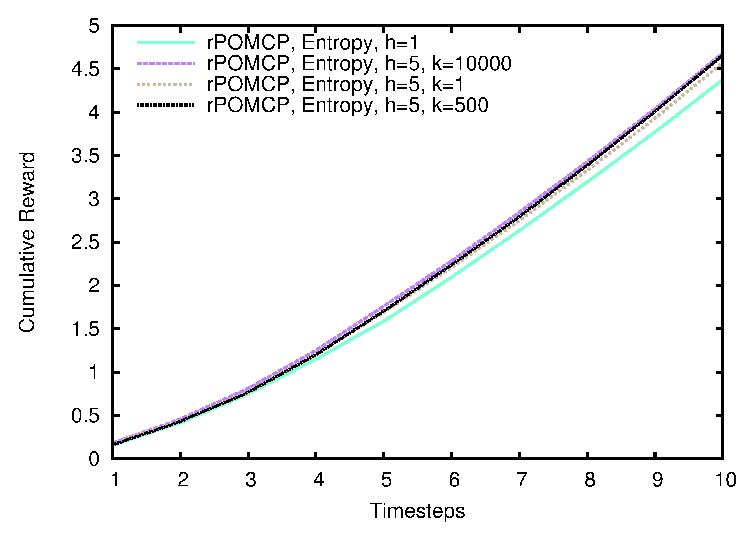
\includegraphics[width=\textwidth]{Images/MyoResults/1e5/E/output}
                \caption{Results in the Myopic World using 1e5 samples and entropy based reward
                function.}
                \label{fig:m5e}
        \end{subfigure}
        ~ %add desired spacing between images, e. g. ~, \quad, \qquad, \hfill etc.
          %(or a blank line to force the subfigure onto a new line)
        \begin{subfigure}[t]{0.3\textwidth}
                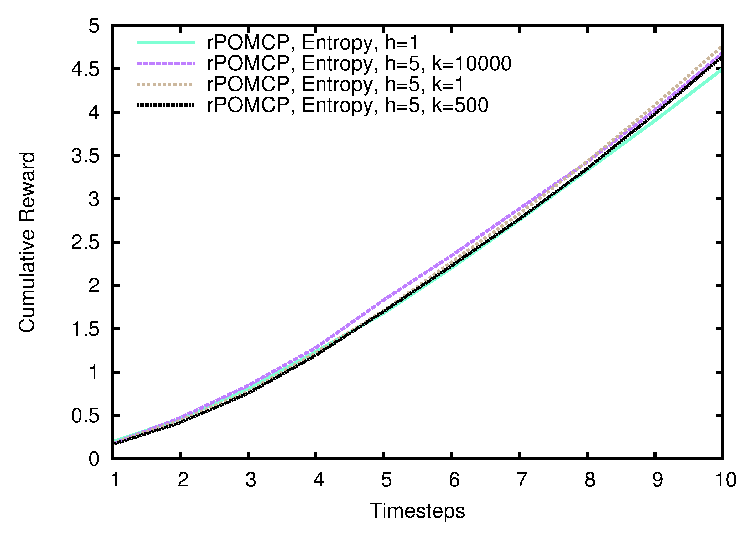
\includegraphics[width=\textwidth]{Images/MyoResults/1e6/E/output}
                \caption{Results in the Myopic World using 1e6 samples and entropy based reward
                function.}
                \label{fig:m6e}
        \end{subfigure}
        \caption{Pictures of animals}\label{fig:me}
\end{figure}

LOTS OF TEXT; LOTS OF TEXT; LOTS OF TEXT; LOTS OF TEXT; LOTS OF TEXT; LOTS OF TEXT; LOTS OF TEXT; LOTS OF TEXT; LOTS OF TEXT; LOTS OF TEXT; LOTS OF TEXT;

\begin{figure}[h]
        \centering
        \begin{subfigure}[t]{0.3\textwidth}
                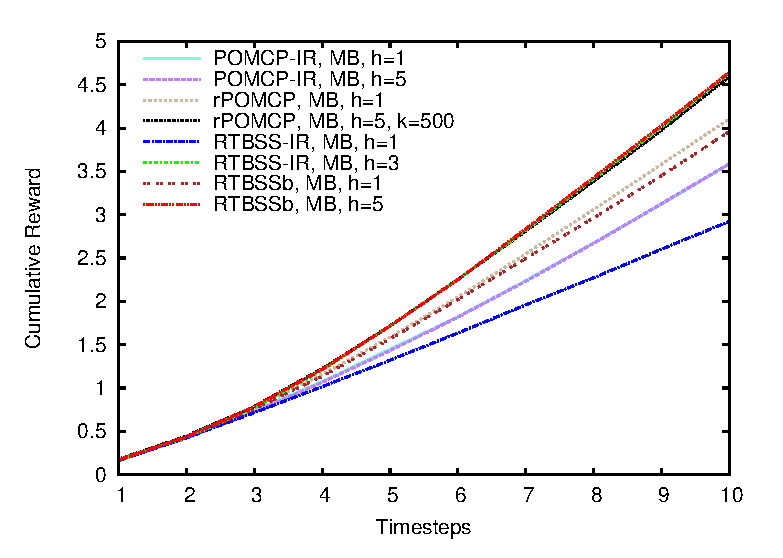
\includegraphics[width=\textwidth]{Images/MyoResults/1e4/MB/output}
                \caption{Results in the Myopic World using 1e4 samples and max-of-belief based
                reward function. RTBSS is not affected by this parameter.}
                \label{fig:m4m}
        \end{subfigure}%
        ~ %add desired spacing between images, e. g. ~, \quad, \qquad, \hfill etc.
          %(or a blank line to force the subfigure onto a new line)
        \begin{subfigure}[t]{0.3\textwidth}
                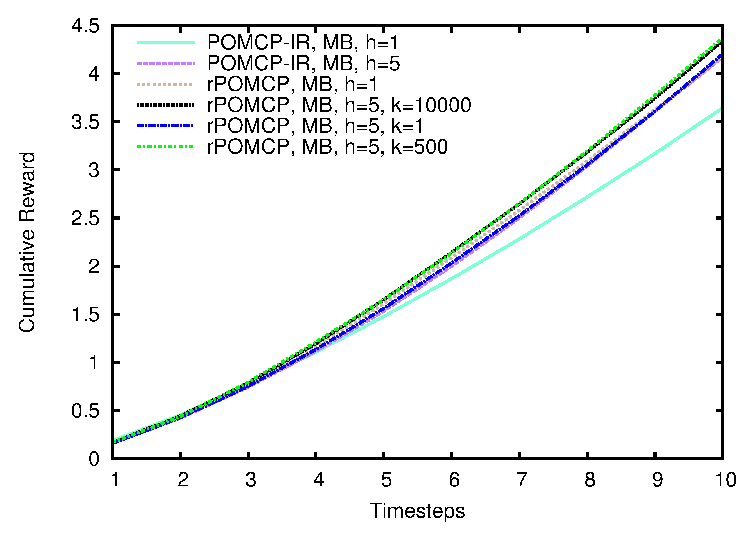
\includegraphics[width=\textwidth]{Images/MyoResults/1e5/MB/output}
                \caption{Results in the Myopic World using 1e4 samples and max-of-belief based
                reward function.}
                \label{fig:m5m}
        \end{subfigure}
        ~ %add desired spacing between images, e. g. ~, \quad, \qquad, \hfill etc.
          %(or a blank line to force the subfigure onto a new line)
        \begin{subfigure}[t]{0.3\textwidth}
                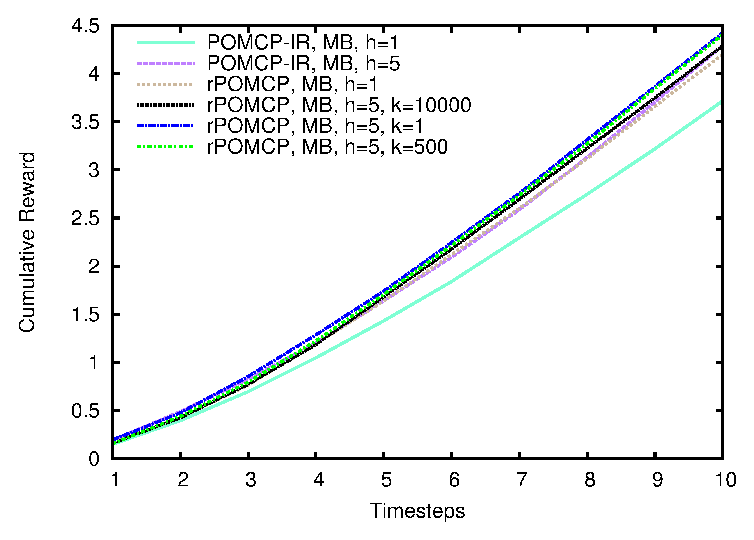
\includegraphics[width=\textwidth]{Images/MyoResults/1e6/MB/output}
                \caption{Results in the Myopic World using 1e4 samples and max-of-belief based
                reward function.}
                \label{fig:m6m}
        \end{subfigure}
        \caption{Pictures of animals}\label{fig:mm}
\end{figure}

\clearpage
\section{Finite Budget}

\begin{figure}[h]
        \centering
        \begin{subfigure}[t]{0.3\textwidth}
                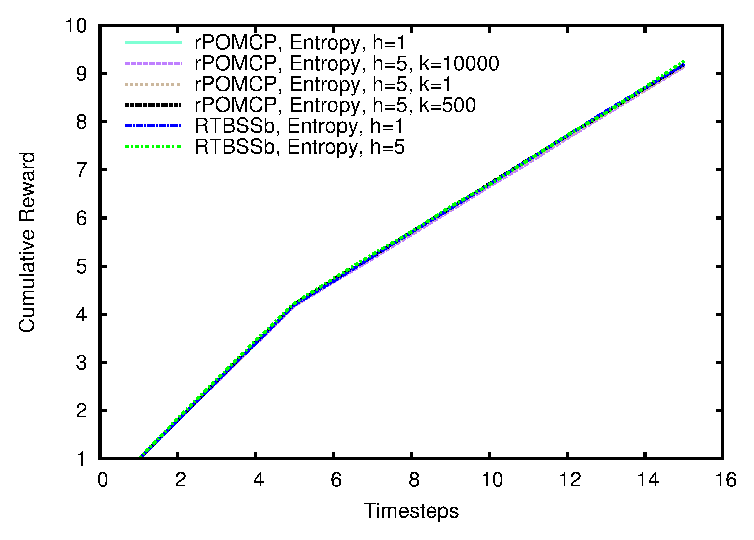
\includegraphics[width=\textwidth]{Images/FiniteBudgetResults/0.5/1e4/E/output}
                \caption{Results in the Finite Budget World using 1e4 samples and entropy based reward
                function. RTBSS is not affected by this parameter.}
                \label{fig:m4e}
        \end{subfigure}%
        ~ %add desired spacing between images, e. g. ~, \quad, \qquad, \hfill etc.
          %(or a blank line to force the subfigure onto a new line)
        \begin{subfigure}[t]{0.3\textwidth}
                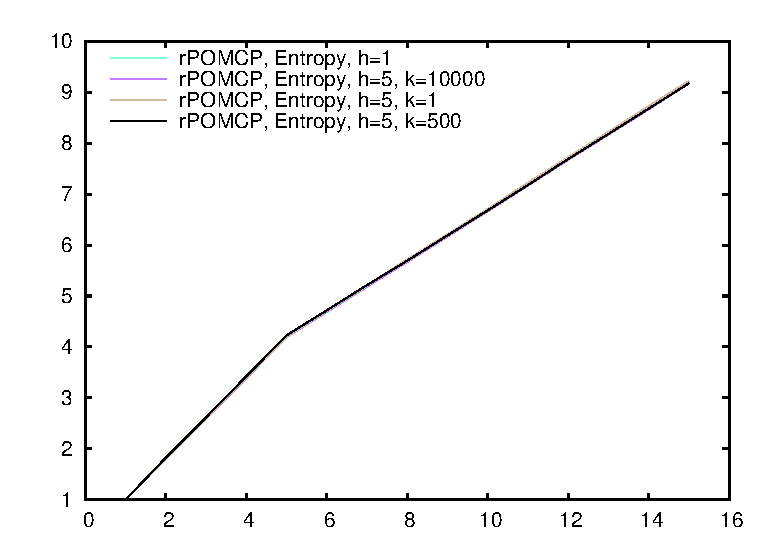
\includegraphics[width=\textwidth]{Images/FiniteBudgetResults/0.5/1e5/E/output}
                \caption{Results in the Finite Budget World using 1e5 samples and entropy based reward
                function.}
                \label{fig:m5e}
        \end{subfigure}
        ~ %add desired spacing between images, e. g. ~, \quad, \qquad, \hfill etc.
          %(or a blank line to force the subfigure onto a new line)
        \begin{subfigure}[t]{0.3\textwidth}
                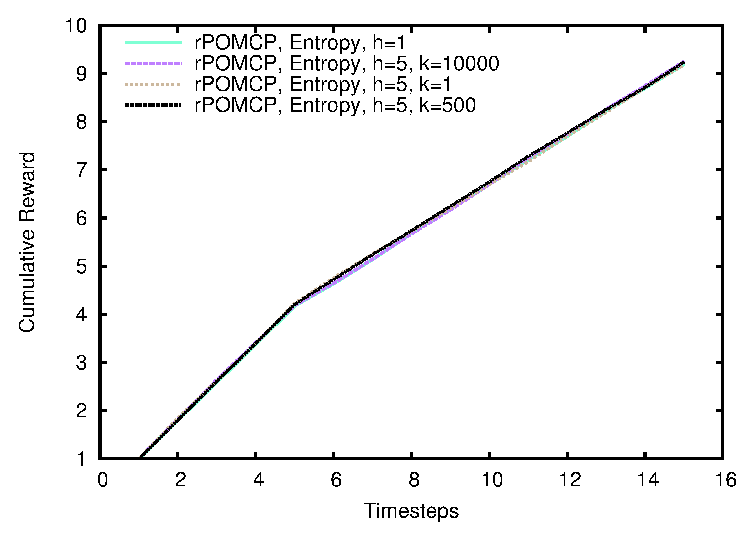
\includegraphics[width=\textwidth]{Images/FiniteBudgetResults/0.5/1e6/E/output}
                \caption{Results in the Finite Budget World using 1e6 samples and entropy based reward
                function.}
                \label{fig:m6e}
        \end{subfigure}
        \caption{Pictures of animals}\label{fig:me}
\end{figure}

LOTS OF TEXT; LOTS OF TEXT; LOTS OF TEXT; LOTS OF TEXT; LOTS OF TEXT; LOTS OF TEXT; LOTS OF TEXT; LOTS OF TEXT; LOTS OF TEXT; LOTS OF TEXT; LOTS OF TEXT;

\begin{figure}[h]
        \centering
        \begin{subfigure}[t]{0.3\textwidth}
                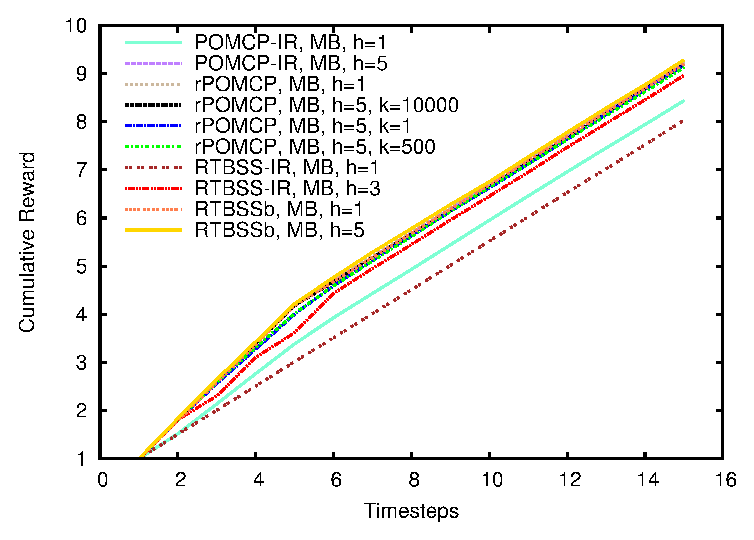
\includegraphics[width=\textwidth]{Images/FiniteBudgetResults/0.5/1e4/MB/output}
                \caption{Results in the Finite Budget World using 1e4 samples and max-of-belief based
                reward function. RTBSS is not affected by this parameter.}
                \label{fig:m4m}
        \end{subfigure}%
        ~ %add desired spacing between images, e. g. ~, \quad, \qquad, \hfill etc.
          %(or a blank line to force the subfigure onto a new line)
        \begin{subfigure}[t]{0.3\textwidth}
                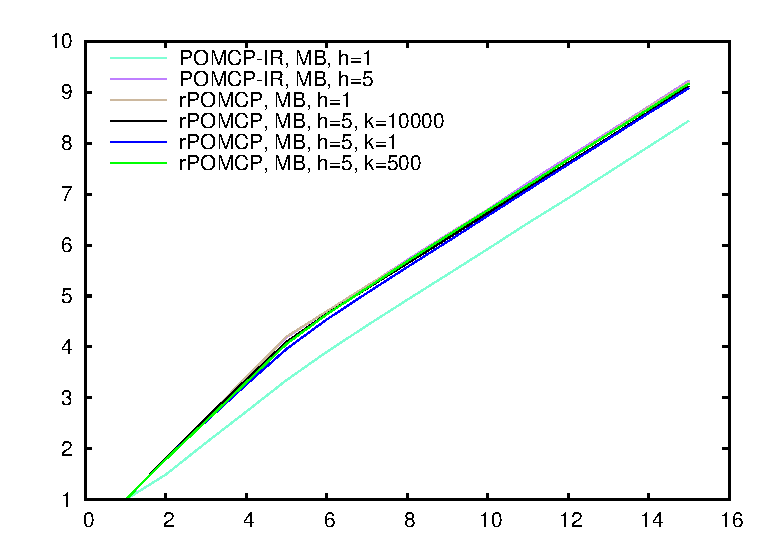
\includegraphics[width=\textwidth]{Images/FiniteBudgetResults/0.5/1e5/MB/output}
                \caption{Results in the Finite Budget World using 1e4 samples and max-of-belief based
                reward function.}
                \label{fig:m5m}
        \end{subfigure}
        ~ %add desired spacing between images, e. g. ~, \quad, \qquad, \hfill etc.
          %(or a blank line to force the subfigure onto a new line)
        \begin{subfigure}[t]{0.3\textwidth}
                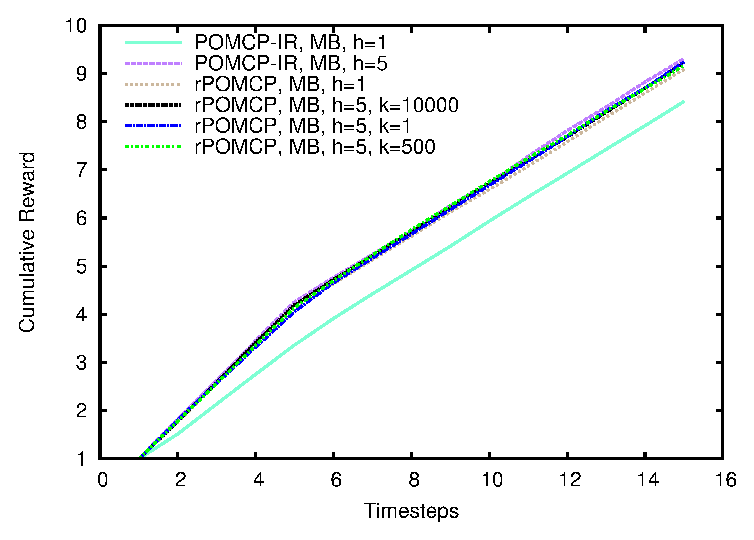
\includegraphics[width=\textwidth]{Images/FiniteBudgetResults/0.5/1e6/MB/output}
                \caption{Results in the Finite Budget World using 1e4 samples and max-of-belief based
                reward function.}
                \label{fig:m6m}
        \end{subfigure}
        \caption{Pictures of animals}\label{fig:mm}
\end{figure}

\begin{figure}[h]
        \centering
        \begin{subfigure}[t]{0.3\textwidth}
                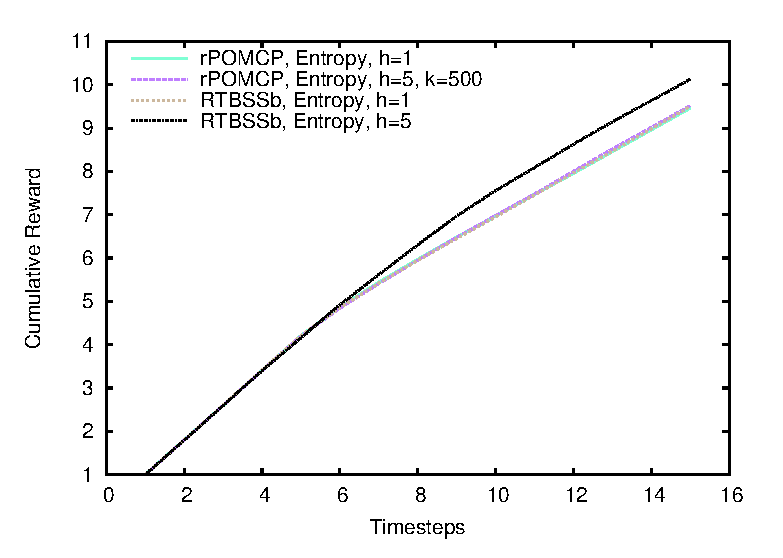
\includegraphics[width=\textwidth]{Images/FiniteBudgetResults/0.75/1e4/E/output}
                \caption{Results in the Finite Budget World using 1e4 samples and entropy based reward
                function. RTBSS is not affected by this parameter.}
                \label{fig:m4e}
        \end{subfigure}%
        ~ %add desired spacing between images, e. g. ~, \quad, \qquad, \hfill etc.
          %(or a blank line to force the subfigure onto a new line)
        \begin{subfigure}[t]{0.3\textwidth}
                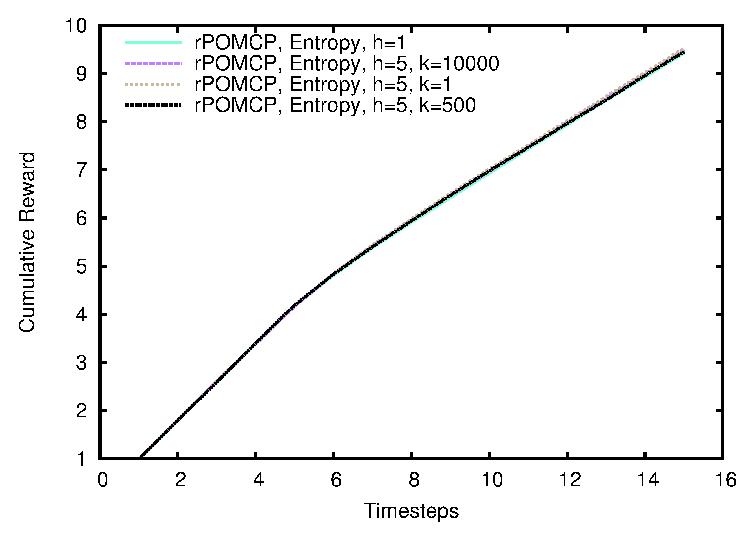
\includegraphics[width=\textwidth]{Images/FiniteBudgetResults/0.75/1e5/E/output}
                \caption{Results in the Finite Budget World using 1e5 samples and entropy based reward
                function.}
                \label{fig:m5e}
        \end{subfigure}
        ~ %add desired spacing between images, e. g. ~, \quad, \qquad, \hfill etc.
          %(or a blank line to force the subfigure onto a new line)
        \begin{subfigure}[t]{0.3\textwidth}
                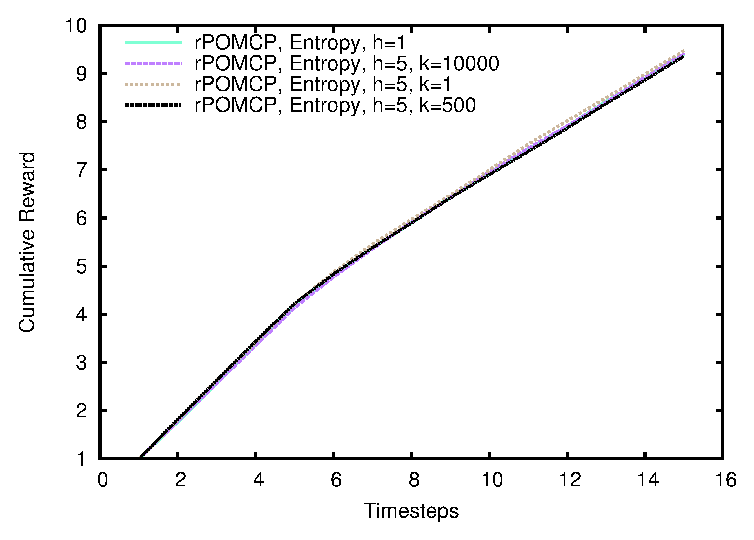
\includegraphics[width=\textwidth]{Images/FiniteBudgetResults/0.75/1e6/E/output}
                \caption{Results in the Finite Budget World using 1e6 samples and entropy based reward
                function.}
                \label{fig:m6e}
        \end{subfigure}
        \caption{Pictures of animals}\label{fig:me}
\end{figure}

LOTS OF TEXT; LOTS OF TEXT; LOTS OF TEXT; LOTS OF TEXT; LOTS OF TEXT; LOTS OF TEXT; LOTS OF TEXT; LOTS OF TEXT; LOTS OF TEXT; LOTS OF TEXT; LOTS OF TEXT;

\begin{figure}[h]
        \centering
        \begin{subfigure}[t]{0.3\textwidth}
                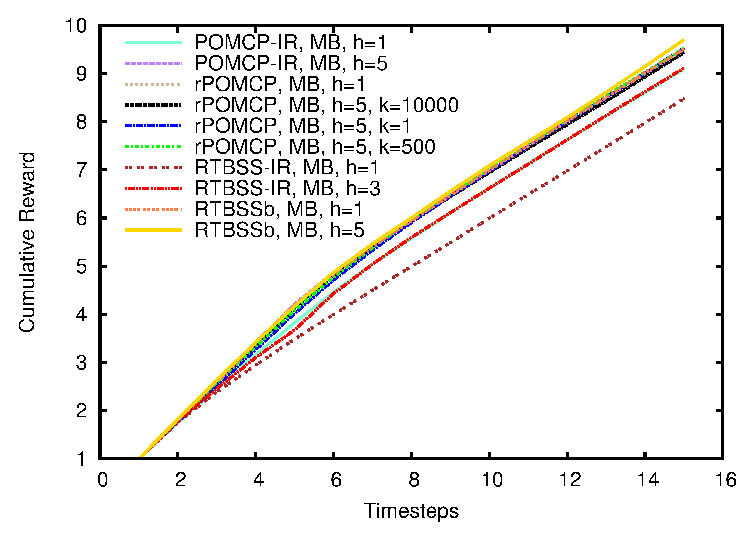
\includegraphics[width=\textwidth]{Images/FiniteBudgetResults/0.75/1e4/MB/output}
                \caption{Results in the Finite Budget World using 1e4 samples and max-of-belief based
                reward function. RTBSS is not affected by this parameter.}
                \label{fig:m4m}
        \end{subfigure}%
        ~ %add desired spacing between images, e. g. ~, \quad, \qquad, \hfill etc.
          %(or a blank line to force the subfigure onto a new line)
        \begin{subfigure}[t]{0.3\textwidth}
                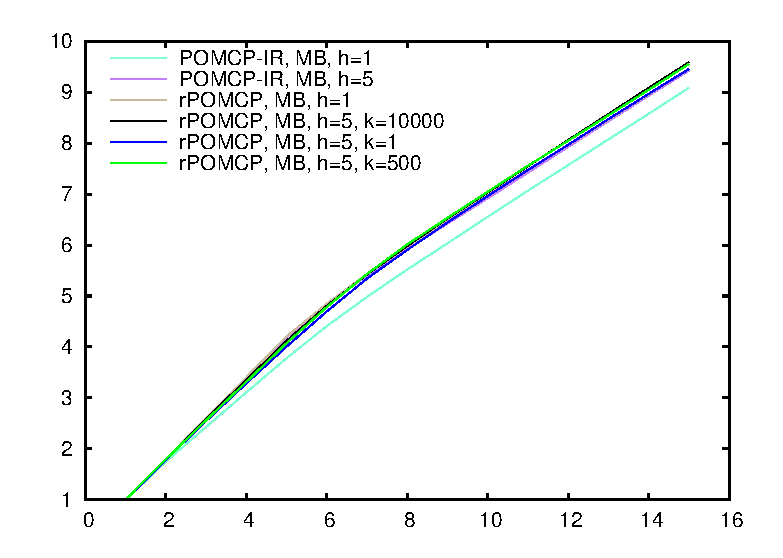
\includegraphics[width=\textwidth]{Images/FiniteBudgetResults/0.75/1e5/MB/output}
                \caption{Results in the Finite Budget World using 1e4 samples and max-of-belief based
                reward function.}
                \label{fig:m5m}
        \end{subfigure}
        ~ %add desired spacing between images, e. g. ~, \quad, \qquad, \hfill etc.
          %(or a blank line to force the subfigure onto a new line)
        \begin{subfigure}[t]{0.3\textwidth}
                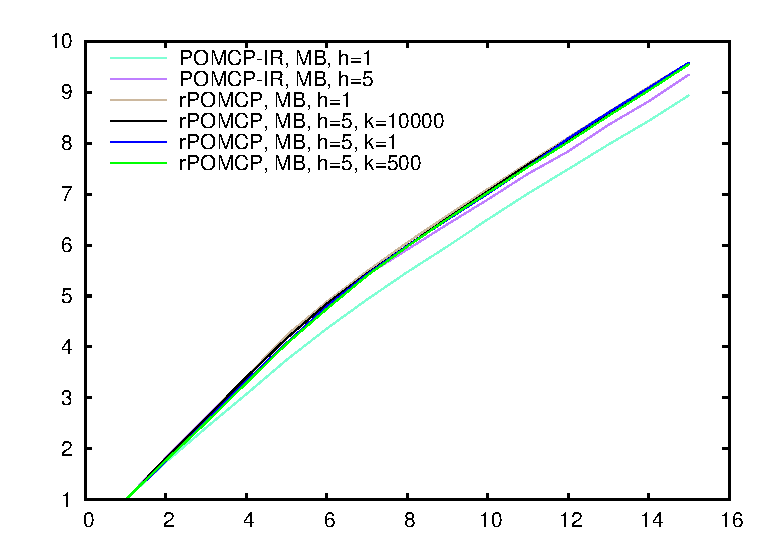
\includegraphics[width=\textwidth]{Images/FiniteBudgetResults/0.75/1e6/MB/output}
                \caption{Results in the Finite Budget World using 1e4 samples and max-of-belief based
                reward function.}
                \label{fig:m6m}
        \end{subfigure}
        \caption{Pictures of animals}\label{fig:mm}
\end{figure}

\clearpage
\section{Camera World}

\begin{figure}[h]
        \centering
        \begin{subfigure}[t]{0.3\textwidth}
                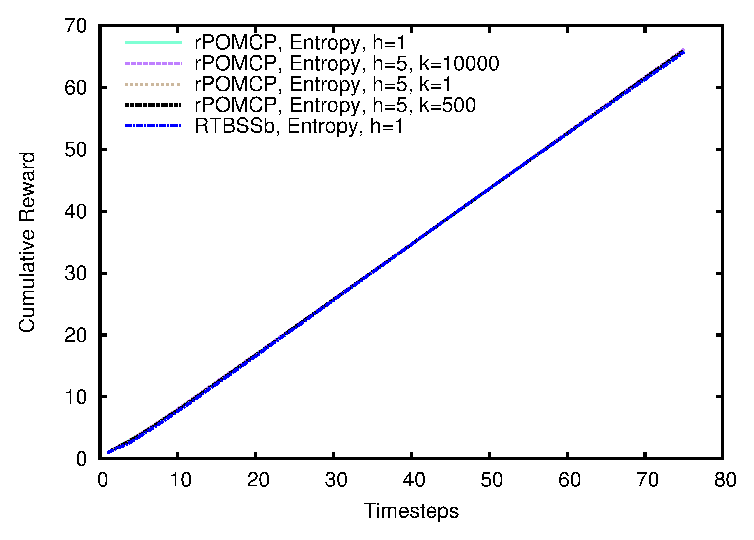
\includegraphics[width=\textwidth]{Images/CameraBasicResults/Small_20x20/1e4/E/output}
                \caption{Results in the Camera World using 1e4 samples and entropy based reward
                function. RTBSS is not affected by this parameter.}
                \label{fig:m4e}
        \end{subfigure}%
        ~ %add desired spacing between images, e. g. ~, \quad, \qquad, \hfill etc.
          %(or a blank line to force the subfigure onto a new line)
        \begin{subfigure}[t]{0.3\textwidth}
                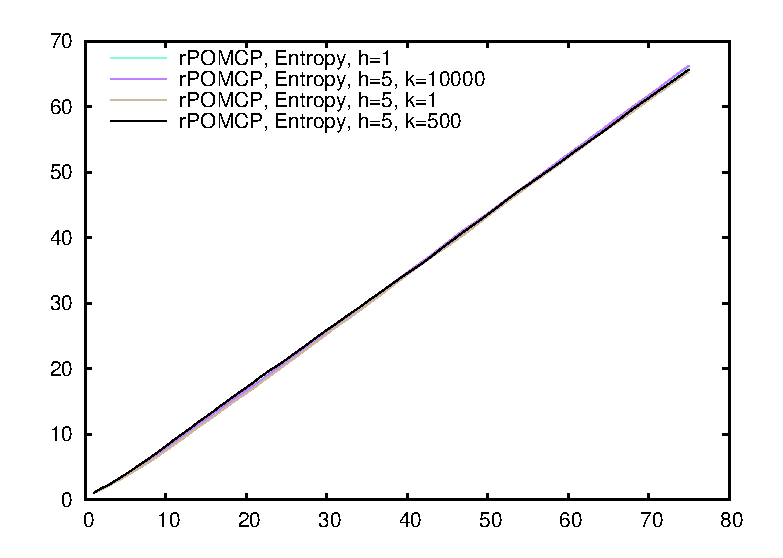
\includegraphics[width=\textwidth]{Images/CameraBasicResults/Small_20x20/1e6/E/output}
                \caption{Results in the Camera World using 1e5 samples and entropy based reward
                function.}
                \label{fig:m5e}
        \end{subfigure}
        ~ %add desired spacing between images, e. g. ~, \quad, \qquad, \hfill etc.
          %(or a blank line to force the subfigure onto a new line)
        \begin{subfigure}[t]{0.3\textwidth}
                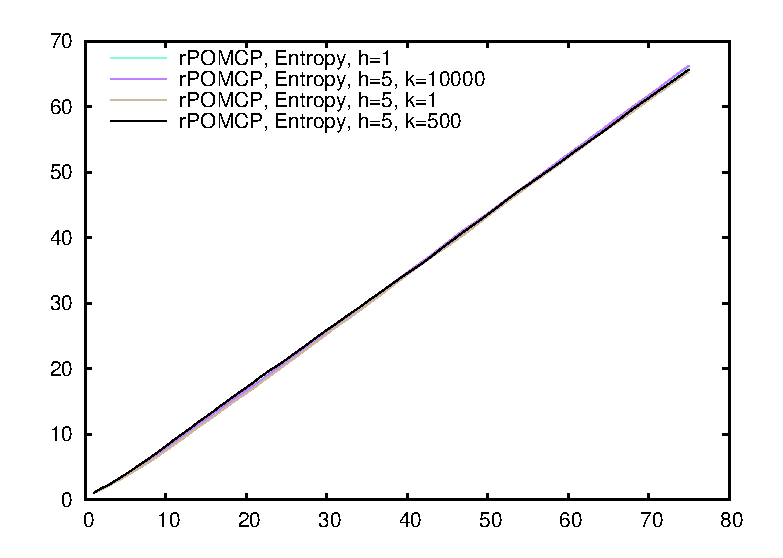
\includegraphics[width=\textwidth]{Images/CameraBasicResults/Small_20x20/1e6/E/output}
                \caption{Results in the Camera World using 1e6 samples and entropy based reward
                function.}
                \label{fig:m6e}
        \end{subfigure}
        \caption{Pictures of animals}\label{fig:me}
\end{figure}

\begin{figure}[h]
        \centering
        \begin{subfigure}[t]{0.3\textwidth}
                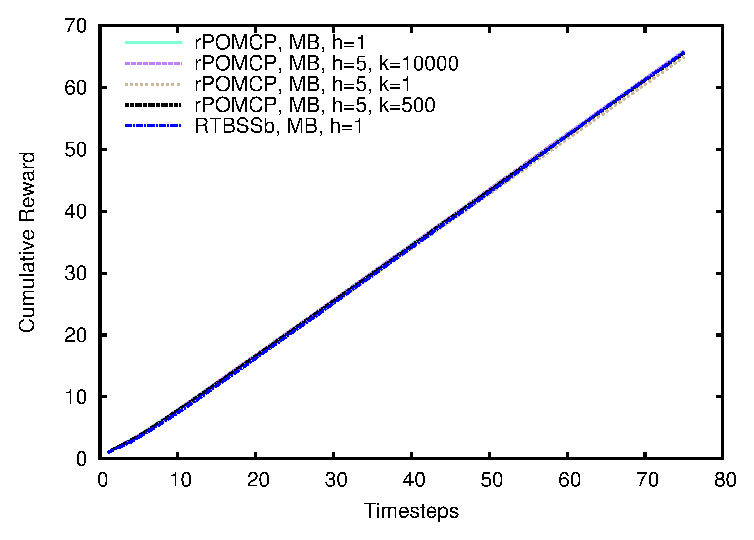
\includegraphics[width=\textwidth]{Images/CameraBasicResults/Small_20x20/1e4/MB/output}
                \caption{Results in the Camera World using 1e4 samples and entropy based reward
                function. RTBSS is not affected by this parameter.}
                \label{fig:m4e}
        \end{subfigure}%
        ~ %add desired spacing between images, e. g. ~, \quad, \qquad, \hfill etc.
          %(or a blank line to force the subfigure onto a new line)
        \begin{subfigure}[t]{0.3\textwidth}
                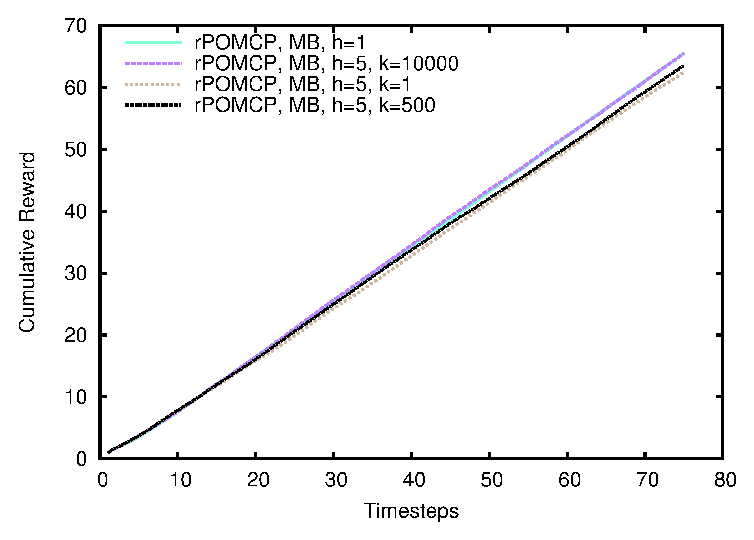
\includegraphics[width=\textwidth]{Images/CameraBasicResults/Small_20x20/1e6/MB/output}
                \caption{Results in the Camera World using 1e5 samples and entropy based reward
                function.}
                \label{fig:m5e}
        \end{subfigure}
        ~ %add desired spacing between images, e. g. ~, \quad, \qquad, \hfill etc.
          %(or a blank line to force the subfigure onto a new line)
        \begin{subfigure}[t]{0.3\textwidth}
                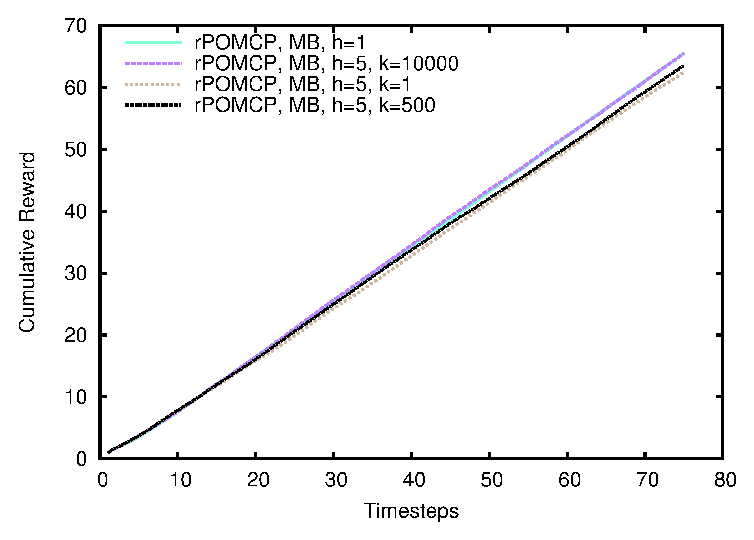
\includegraphics[width=\textwidth]{Images/CameraBasicResults/Small_20x20/1e6/MB/output}
                \caption{Results in the Camera World using 1e6 samples and entropy based reward
                function.}
                \label{fig:m6e}
        \end{subfigure}
        \caption{Pictures of animals}\label{fig:me}
\end{figure}

\begin{figure}[h]
        \centering
        \begin{subfigure}[t]{0.3\textwidth}
                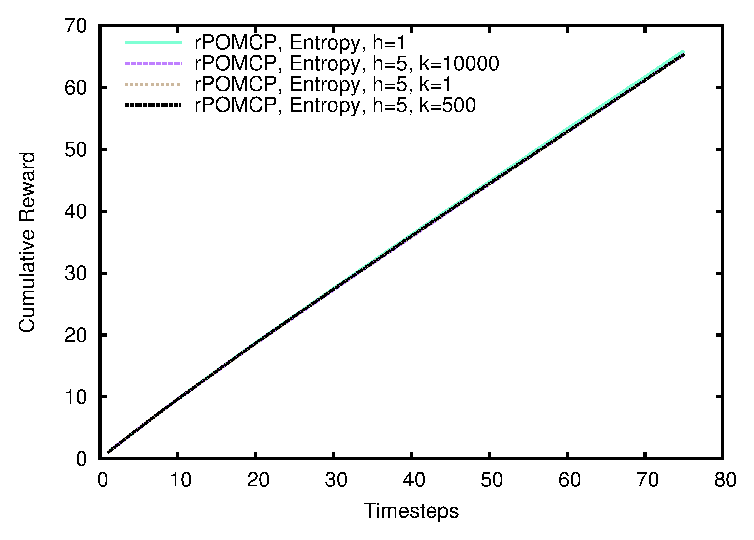
\includegraphics[width=\textwidth]{Images/CameraBasicResults/Big_50x50/1e4/E/output}
                \caption{Results in the Camera World using 1e4 samples and entropy based reward
                function. RTBSS is not affected by this parameter.}
                \label{fig:m4e}
        \end{subfigure}%
        ~ %add desired spacing between images, e. g. ~, \quad, \qquad, \hfill etc.
          %(or a blank line to force the subfigure onto a new line)
        \begin{subfigure}[t]{0.3\textwidth}
                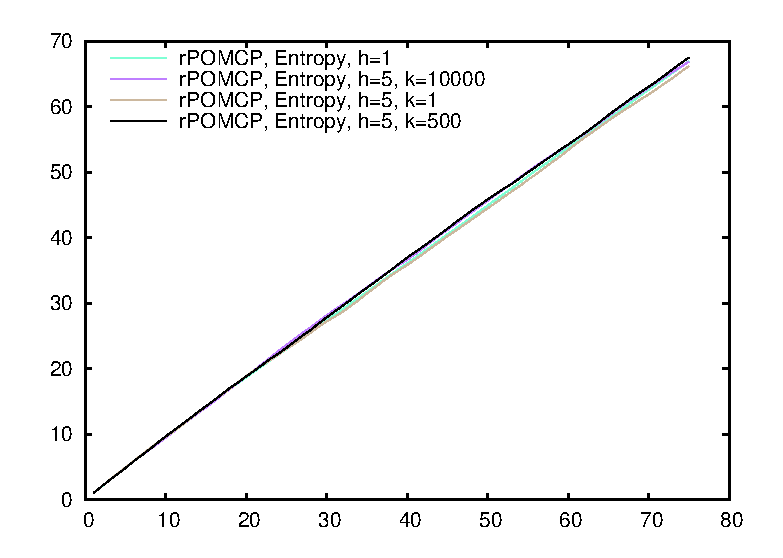
\includegraphics[width=\textwidth]{Images/CameraBasicResults/Big_50x50/1e6/E/output}
                \caption{Results in the Camera World using 1e5 samples and entropy based reward
                function.}
                \label{fig:m5e}
        \end{subfigure}
        ~ %add desired spacing between images, e. g. ~, \quad, \qquad, \hfill etc.
          %(or a blank line to force the subfigure onto a new line)
        \begin{subfigure}[t]{0.3\textwidth}
                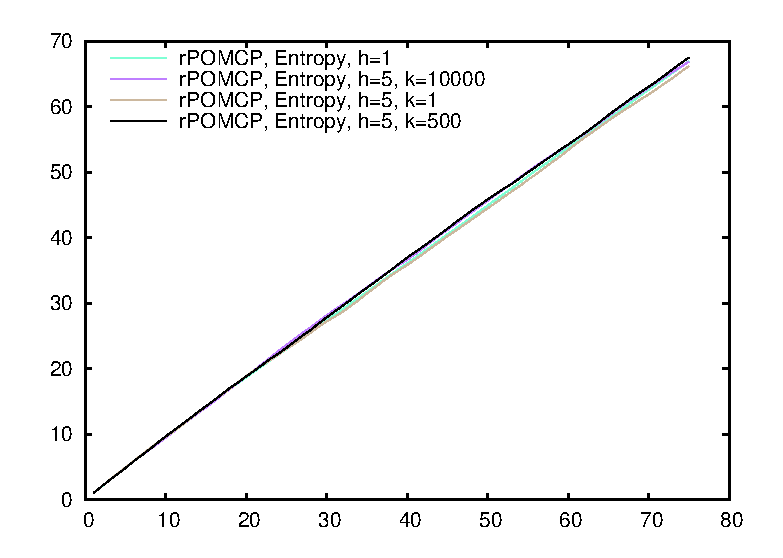
\includegraphics[width=\textwidth]{Images/CameraBasicResults/Big_50x50/1e6/E/output}
                \caption{Results in the Camera World using 1e6 samples and entropy based reward
                function.}
                \label{fig:m6e}
        \end{subfigure}
        \caption{Pictures of animals}\label{fig:me}
\end{figure}

\begin{figure}[h]
        \centering
        \begin{subfigure}[t]{0.3\textwidth}
                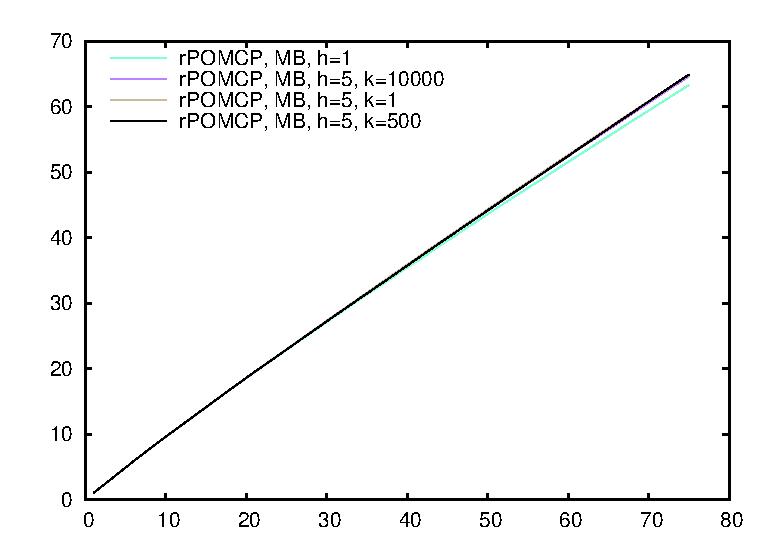
\includegraphics[width=\textwidth]{Images/CameraBasicResults/Big_50x50/1e4/MB/output}
                \caption{Results in the Camera World using 1e4 samples and entropy based reward
                function. RTBSS is not affected by this parameter.}
                \label{fig:m4e}
        \end{subfigure}%
        ~ %add desired spacing between images, e. g. ~, \quad, \qquad, \hfill etc.
          %(or a blank line to force the subfigure onto a new line)
        \begin{subfigure}[t]{0.3\textwidth}
                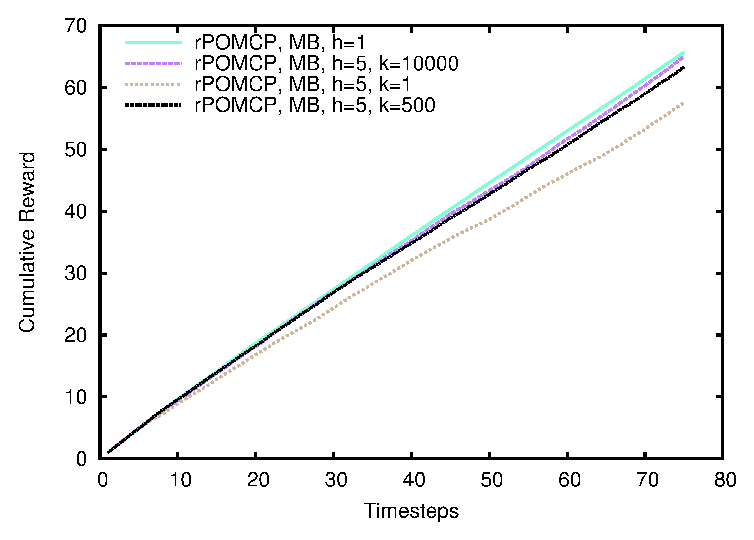
\includegraphics[width=\textwidth]{Images/CameraBasicResults/Big_50x50/1e6/MB/output}
                \caption{Results in the Camera World using 1e5 samples and entropy based reward
                function.}
                \label{fig:m5e}
        \end{subfigure}
        ~ %add desired spacing between images, e. g. ~, \quad, \qquad, \hfill etc.
          %(or a blank line to force the subfigure onto a new line)
        \begin{subfigure}[t]{0.3\textwidth}
                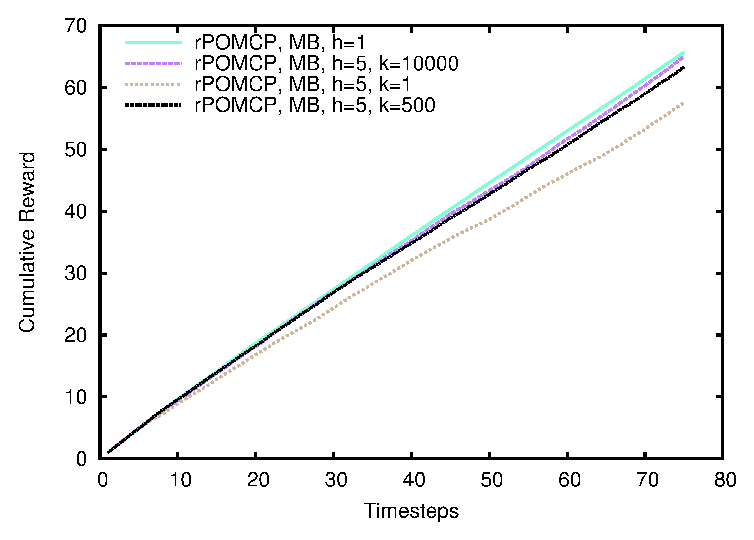
\includegraphics[width=\textwidth]{Images/CameraBasicResults/Big_50x50/1e6/MB/output}
                \caption{Results in the Camera World using 1e6 samples and entropy based reward
                function.}
                \label{fig:m6e}
        \end{subfigure}
        \caption{Pictures of animals}\label{fig:me}
\end{figure}

\begin{figure}[h]
        \centering
        \begin{subfigure}[t]{0.5\textwidth}
                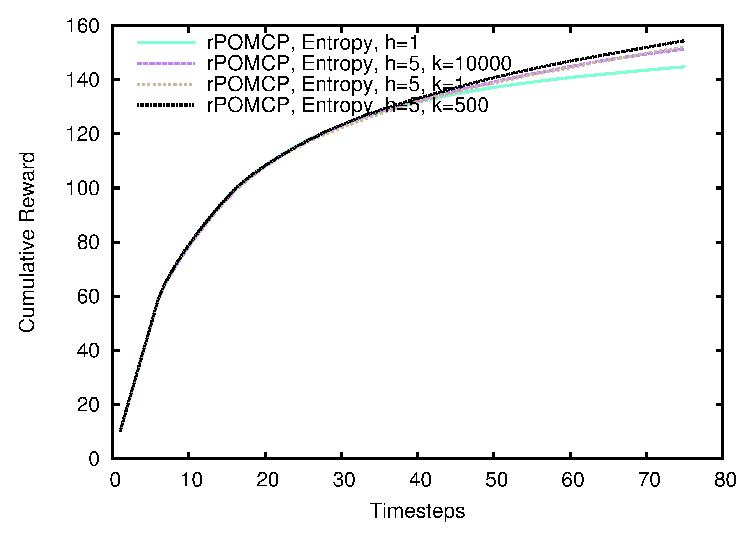
\includegraphics[width=\textwidth]{Images/CameraBasicResults/Big_50x50/Multi/E/output}
                \caption{Results in the Camera World using 1e4 samples and entropy based reward
                function. RTBSS is not affected by this parameter.}
                \label{fig:m4e}
        \end{subfigure}%
        ~ %add desired spacing between images, e. g. ~, \quad, \qquad, \hfill etc.
          %(or a blank line to force the subfigure onto a new line)
        \begin{subfigure}[t]{0.5\textwidth}
                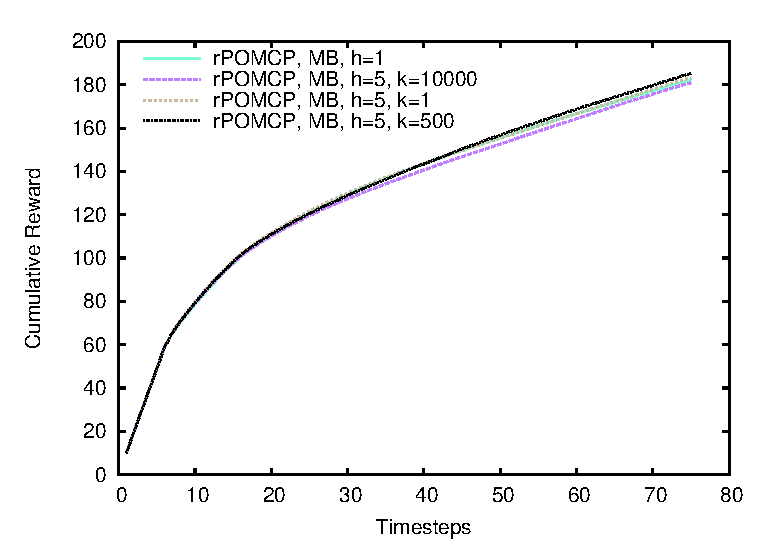
\includegraphics[width=\textwidth]{Images/CameraBasicResults/Big_50x50/Multi/MB/output}
                \caption{Results in the Camera World using 1e5 samples and entropy based reward
                function.}
                \label{fig:m5e}
        \end{subfigure}
        \caption{Pictures of animals}\label{fig:me}
\end{figure}

\begin{figure}[h]
        \centering
        \begin{subfigure}[t]{0.3\textwidth}
                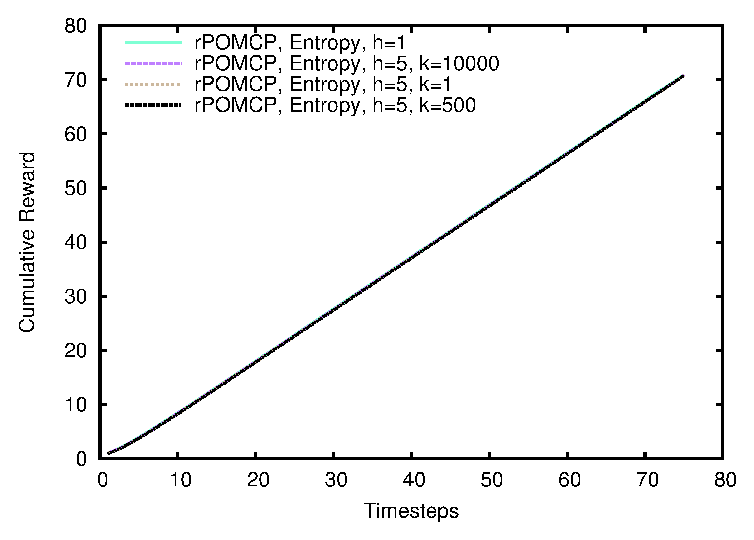
\includegraphics[width=\textwidth]{Images/CameraPathResults/Small_20x20/1e4/E/output}
                \caption{Results in the Camera World using 1e4 samples and entropy based reward
                function. RTBSS is not affected by this parameter.}
                \label{fig:m4e}
        \end{subfigure}%
        ~ %add desired spacing between images, e. g. ~, \quad, \qquad, \hfill etc.
          %(or a blank line to force the subfigure onto a new line)
        \begin{subfigure}[t]{0.3\textwidth}
                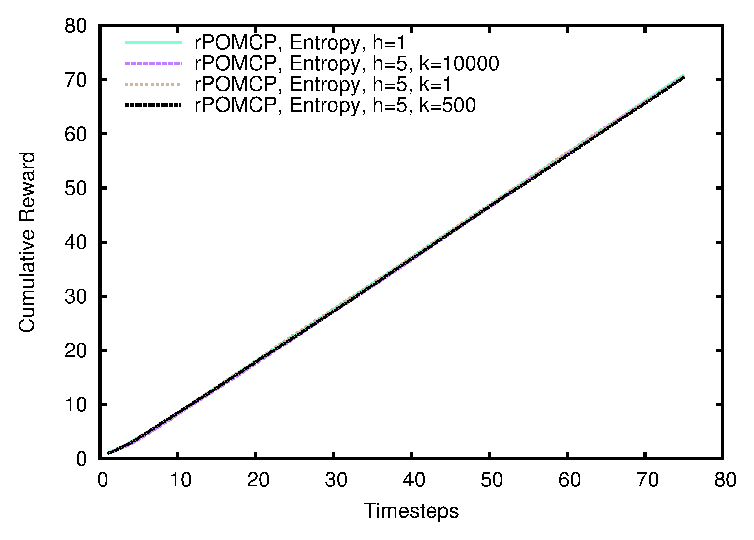
\includegraphics[width=\textwidth]{Images/CameraPathResults/Small_20x20/1e6/E/output}
                \caption{Results in the Camera World using 1e5 samples and entropy based reward
                function.}
                \label{fig:m5e}
        \end{subfigure}
        ~ %add desired spacing between images, e. g. ~, \quad, \qquad, \hfill etc.
          %(or a blank line to force the subfigure onto a new line)
        \begin{subfigure}[t]{0.3\textwidth}
                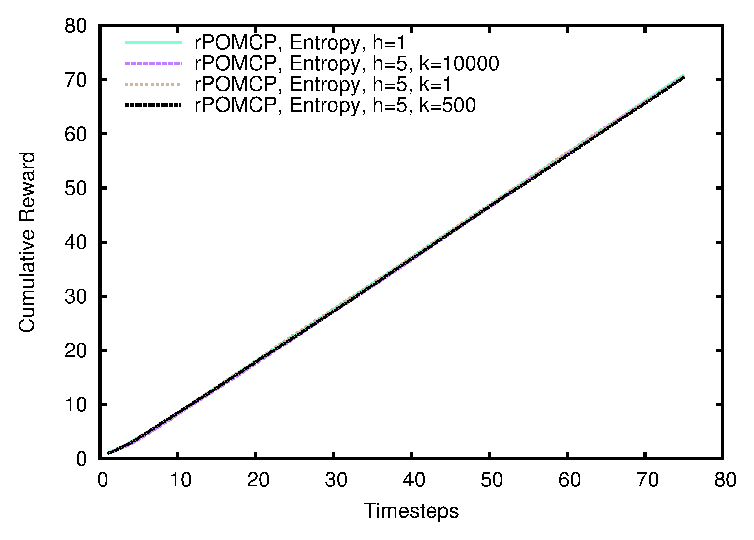
\includegraphics[width=\textwidth]{Images/CameraPathResults/Small_20x20/1e6/E/output}
                \caption{Results in the Camera World using 1e6 samples and entropy based reward
                function.}
                \label{fig:m6e}
        \end{subfigure}
        \caption{Pictures of animals}\label{fig:me}
\end{figure}

\begin{figure}[h]
        \centering
        \begin{subfigure}[t]{0.3\textwidth}
                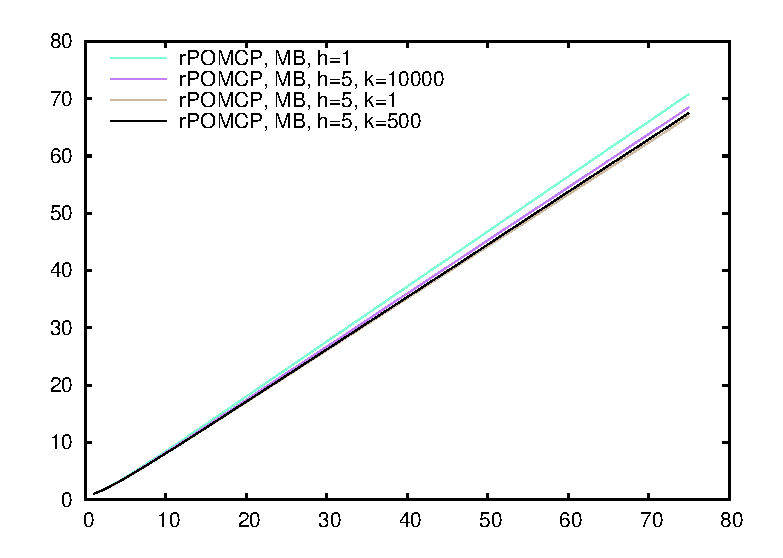
\includegraphics[width=\textwidth]{Images/CameraPathResults/Small_20x20/1e4/MB/output}
                \caption{Results in the Camera World using 1e4 samples and entropy based reward
                function. RTBSS is not affected by this parameter.}
                \label{fig:m4e}
        \end{subfigure}%
        ~ %add desired spacing between images, e. g. ~, \quad, \qquad, \hfill etc.
          %(or a blank line to force the subfigure onto a new line)
        \begin{subfigure}[t]{0.3\textwidth}
                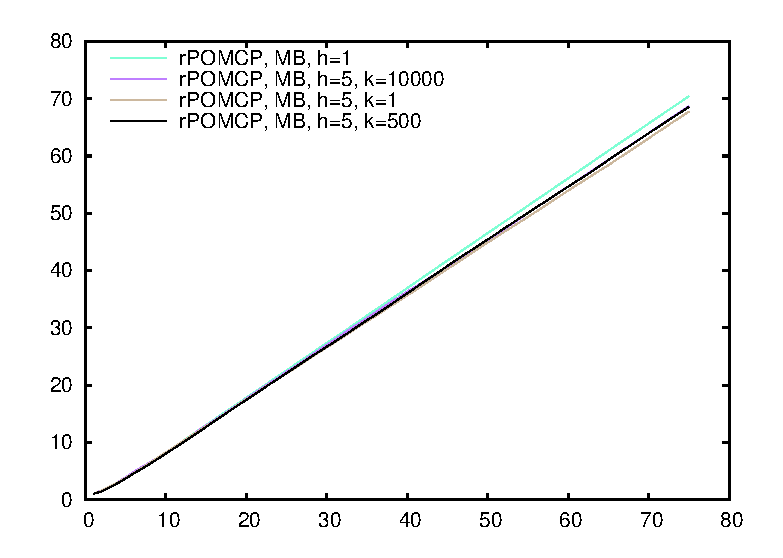
\includegraphics[width=\textwidth]{Images/CameraPathResults/Small_20x20/1e6/MB/output}
                \caption{Results in the Camera World using 1e5 samples and entropy based reward
                function.}
                \label{fig:m5e}
        \end{subfigure}
        ~ %add desired spacing between images, e. g. ~, \quad, \qquad, \hfill etc.
          %(or a blank line to force the subfigure onto a new line)
        \begin{subfigure}[t]{0.3\textwidth}
                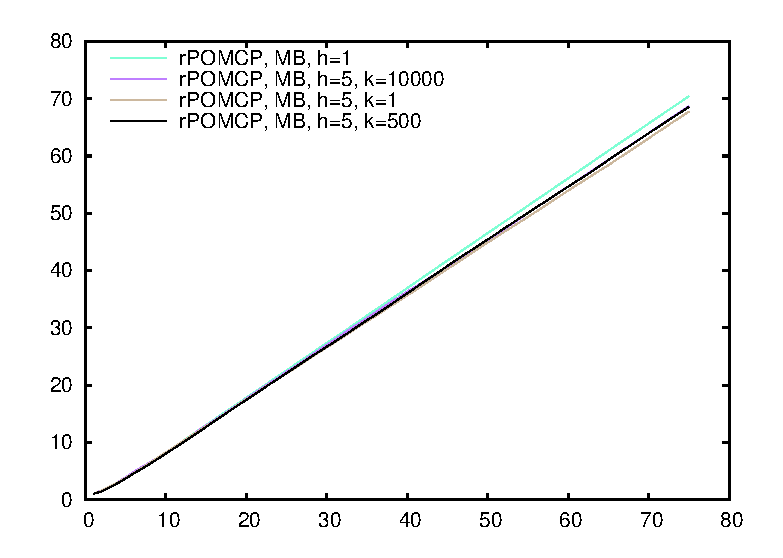
\includegraphics[width=\textwidth]{Images/CameraPathResults/Small_20x20/1e6/MB/output}
                \caption{Results in the Camera World using 1e6 samples and entropy based reward
                function.}
                \label{fig:m6e}
        \end{subfigure}
        \caption{Pictures of animals}\label{fig:me}
\end{figure}

\begin{figure}[h]
        \centering
        \begin{subfigure}[t]{0.3\textwidth}
                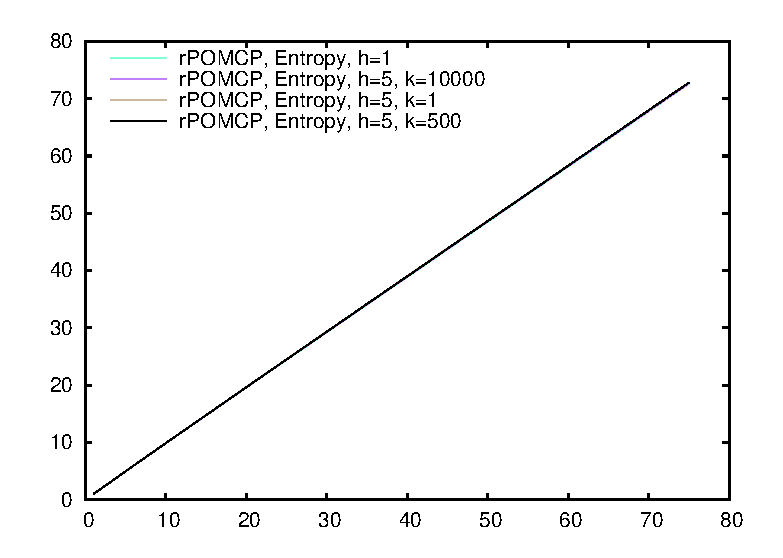
\includegraphics[width=\textwidth]{Images/CameraPathResults/Big_50x50/1e4/E/output}
                \caption{Results in the Camera World using 1e4 samples and entropy based reward
                function. RTBSS is not affected by this parameter.}
                \label{fig:m4e}
        \end{subfigure}%
        ~ %add desired spacing between images, e. g. ~, \quad, \qquad, \hfill etc.
          %(or a blank line to force the subfigure onto a new line)
        \begin{subfigure}[t]{0.3\textwidth}
                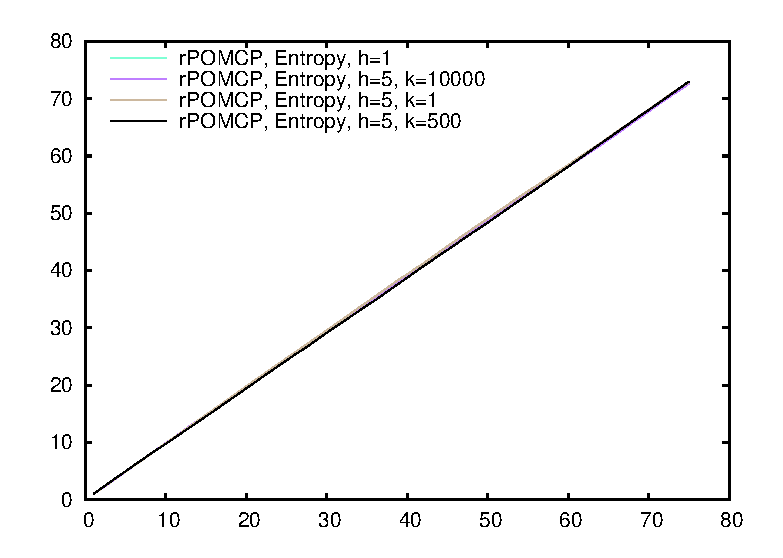
\includegraphics[width=\textwidth]{Images/CameraPathResults/Big_50x50/1e6/E/output}
                \caption{Results in the Camera World using 1e5 samples and entropy based reward
                function.}
                \label{fig:m5e}
        \end{subfigure}
        ~ %add desired spacing between images, e. g. ~, \quad, \qquad, \hfill etc.
          %(or a blank line to force the subfigure onto a new line)
        \begin{subfigure}[t]{0.3\textwidth}
                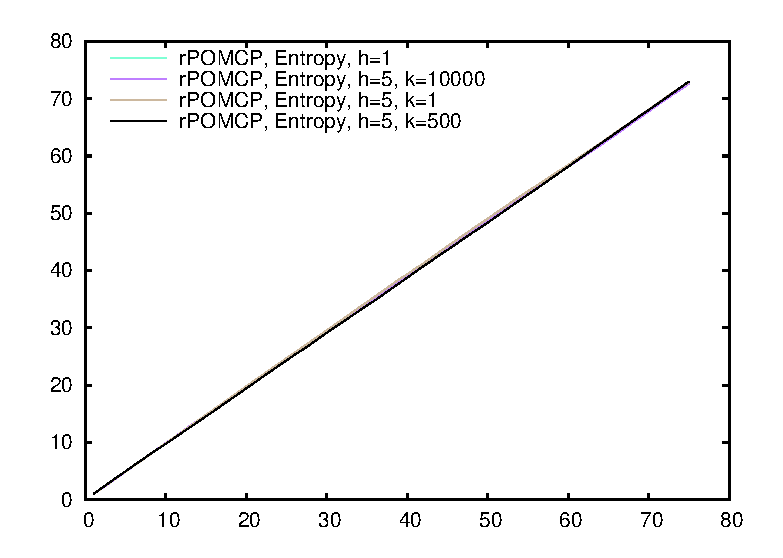
\includegraphics[width=\textwidth]{Images/CameraPathResults/Big_50x50/1e6/E/output}
                \caption{Results in the Camera World using 1e6 samples and entropy based reward
                function.}
                \label{fig:m6e}
        \end{subfigure}
        \caption{Pictures of animals}\label{fig:me}
\end{figure}

\begin{figure}[h]
        \centering
        \begin{subfigure}[t]{0.3\textwidth}
                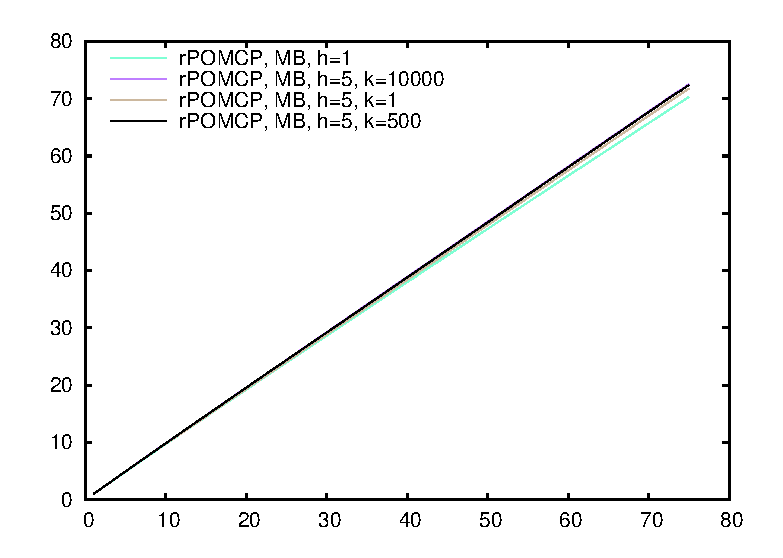
\includegraphics[width=\textwidth]{Images/CameraPathResults/Big_50x50/1e4/MB/output}
                \caption{Results in the Camera World using 1e4 samples and entropy based reward
                function. RTBSS is not affected by this parameter.}
                \label{fig:m4e}
        \end{subfigure}%
        ~ %add desired spacing between images, e. g. ~, \quad, \qquad, \hfill etc.
          %(or a blank line to force the subfigure onto a new line)
        \begin{subfigure}[t]{0.3\textwidth}
                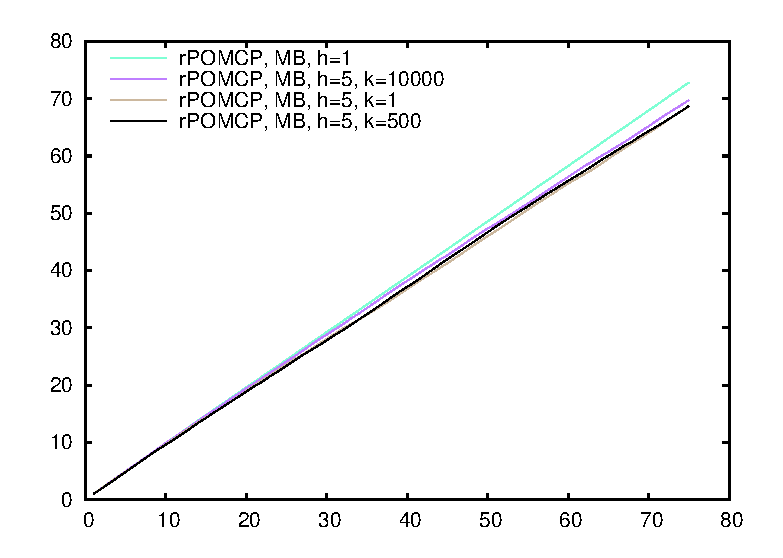
\includegraphics[width=\textwidth]{Images/CameraPathResults/Big_50x50/1e6/MB/output}
                \caption{Results in the Camera World using 1e5 samples and entropy based reward
                function.}
                \label{fig:m5e}
        \end{subfigure}
        ~ %add desired spacing between images, e. g. ~, \quad, \qquad, \hfill etc.
          %(or a blank line to force the subfigure onto a new line)
        \begin{subfigure}[t]{0.3\textwidth}
                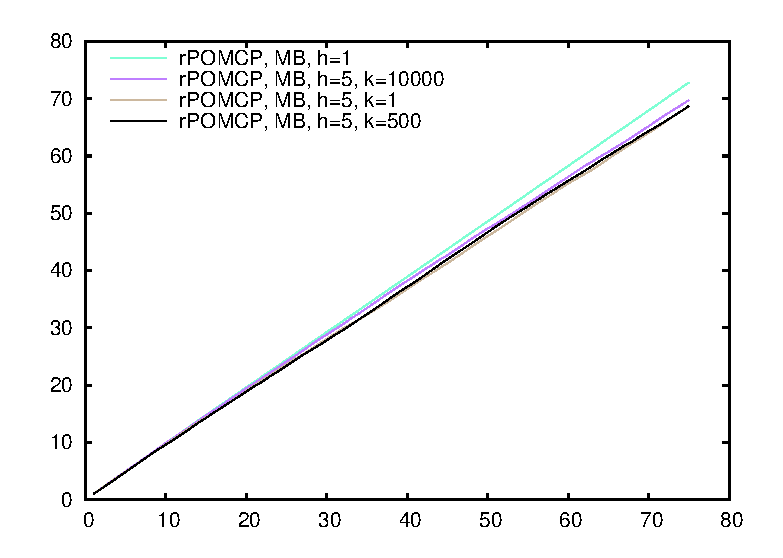
\includegraphics[width=\textwidth]{Images/CameraPathResults/Big_50x50/1e6/MB/output}
                \caption{Results in the Camera World using 1e6 samples and entropy based reward
                function.}
                \label{fig:m6e}
        \end{subfigure}
        \caption{Pictures of animals}\label{fig:me}
\end{figure}

\begin{figure}[h]
        \centering
        \begin{subfigure}[t]{0.5\textwidth}
                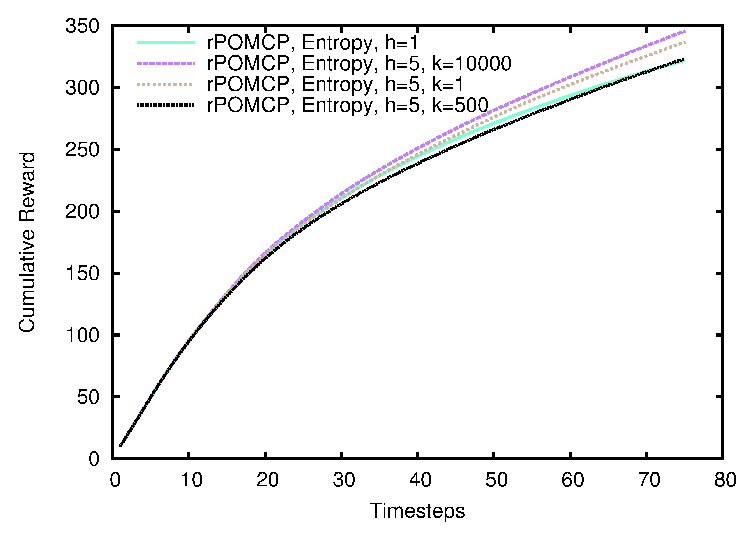
\includegraphics[width=\textwidth]{Images/CameraPathResults/Big_50x50/Multi/E/output}
                \caption{Results in the Camera World using 1e4 samples and entropy based reward
                function. RTBSS is not affected by this parameter.}
                \label{fig:m4e}
        \end{subfigure}%
        ~ %add desired spacing between images, e. g. ~, \quad, \qquad, \hfill etc.
          %(or a blank line to force the subfigure onto a new line)
        \begin{subfigure}[t]{0.5\textwidth}
                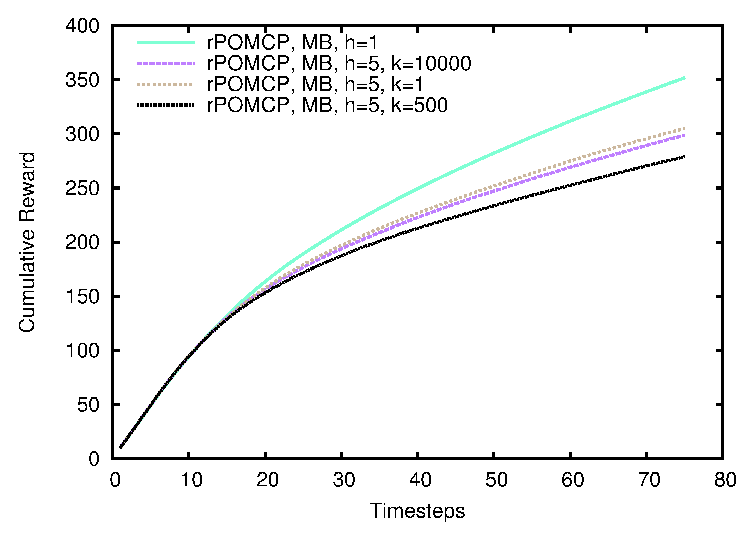
\includegraphics[width=\textwidth]{Images/CameraPathResults/Big_50x50/Multi/MB/output}
                \caption{Results in the Camera World using 1e5 samples and entropy based reward
                function.}
                \label{fig:m5e}
        \end{subfigure}
        \caption{Pictures of animals}\label{fig:me}
\end{figure}


\chapter{Conclusion}\label{ref:conclusion}
In this thesis we tackle active perception for resource allocation in multi-camera systems. In
particular, we try to track a number of targets over an extended period of time, while trying to
make an optimal usage of available resources under specific constraints, namely partial
observability, environment size and limited access to cameras.

In order to fulfill our goal we have improved over POMCP \cite{cit:pomcp} in order to fit our
particular prerequisites, removing shortcomings which prevented its application in our setting.
Starting from the POMCP algorithm, which uses online Monte Carlo techniques to approximately plan in
POMDP models, we have extended it in order to be applied to belief-based POMDPs, called
$\rho$POMDPs, using entropy or max-of-belief as reward functions. Our approach, called $\rho$POMCP,
can tackle problems orders of magnitude bigger than existing alternatives and can be applied to all
$\rho$POMDP problems, not only those proposed in this work.

$\rho$POMCP achieves these results by estimating the belief-based reward function directly on the
particle beliefs, without the need for full beliefs to be propagated within the search tree. In
addition each updated estimate can be cheaply backpropagated up in the tree substituting previous
estimates, guaranteeing that the UCT process always uses the most current available information in
order to select the best available action. The method does not require significant additional
computation with respect to the original method POMCP, which allows it to be applied to large sized
problems.

We have compared our approach to already existing methods, and shown the differences in performance
between them. In particular, $\rho$POMCP can scale successfully on problems orders of magnitude
bigger than what was possible with previous approaches, and can be used to track multiple targets
concurrently in a very effective and parallelizable manner. Our approach can be easily distributed
between separate computing nodes, and the amount of information and bandwidth that needs to be
shared between any such nodes is very limited.

At the same time, our results indicate that while theoretically non-myopic solutions are sometimes
necessary for optimal solutions in active perception, in a multi-camera system setting the added
overhead required by planning over more than a single timestep may not be justified by the
additional gained rewards - if the model of the environment even allows for any. This seems to
replicate results obtained by \cite{cit:relworktanks}, which show that planning for more than one
timestep in a realistic setting does not seem to improve effectiveness much, while it is needed when
the problem is artificially constrained so to require forethinking by the agent.

\section{Future Work}

Additional efforts may be useful in order to evaluate the effectiveness of our method on
$\rho$POMDPs where actions actually do influence the environment. In such cases the value in
planning for the future and avoiding a myopic approach is increased as the agent's actions need to
be selected taking into consideration how the environment will change with respect to the agent's
choice.

Another improvement would be to extend our reward approximations with respect to reward functions
other than entropy and max-of-belief.


\nocite{*}
\appendix

\chapter{Myopicity of Active Perception}\label{ref:appendix_proof}
POMDPs can be used naturally to compute non-myopic policies to solve a particular task. We show here
that some Active Perception tasks require the usage of non-myopic solutions to achieve optimality,
and thus we can use POMDPs to model efficiently such tasks.

We propose two different POMDP models of Active Perception problems. For one of the models we will
prove that a non-myopic solution is required in order to obtain an optimal solution. For the second
we will prove that a non-myopic solution is not required. The results we show are for both max of
belief and negative entropy reward functions.

\section{Non-Myopic World}

Let's consider a world where the agent is tasked with tracking a single person that is walking. The
person can, at any moment, be in one of a series of rooms, and can transition between them. In each
room there is a camera which can observe the room itself and nothing else. If the agent activates
the camera situated in a room the person just entered there is a $0.8$ probability that the agent will
obtain a ``found'' observation, and a $0.2$ probability that it will obtain a ``null'' observation.
On the other hand, if the agent activates any other camera, it will obtain a ``null'' observation
with $0.8$ probability and a ``found'' observation with $0.2$ probability. Each time a camera is
activated, the person will move to another accessible room. The agent's goal is to guess correctly
where the person has moved for two times in a row, knowing only that at the start the person could
be in any room.

We will now create an instance of the problem we have just finished describing. Let's now suppose
that in our world there are 6 rooms, and we know that the person will transition from one to another
with the following probabilities:

\begin{center}
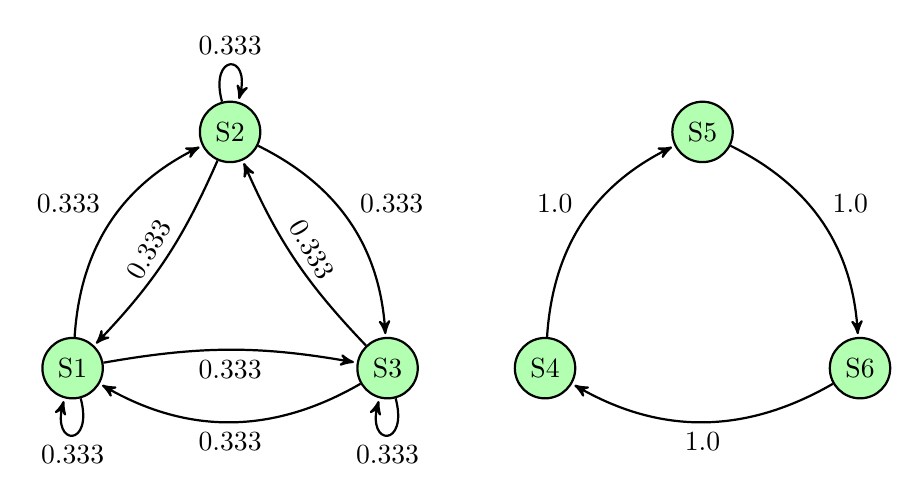
\begin{tikzpicture}[->,>=stealth',shorten >=1pt,auto,node distance=4cm,thick,main node/.style={circle,draw,font=\Large\bfseries}]
\tikzstyle{state} = [circle, draw=black, fill=green!30]
\tikzstyle{arrow} = [thick,->,>=stealth]

\node (s1) at (0,0) [state] {S1};
\node (s2) at (2,3) [state] {S2};
\node (s3) at (4,0) [state] {S3};
\node (s4) at (6,0) [state] {S4};
\node (s5) at (8,3) [state] {S5};
\node (s6) at (10,0) [state] {S6};

\path
    (s1) edge [loop below] node {0.333} (s1)
         edge [bend left] node {0.333} (s2)
         edge [bend left=10] node[below] {0.333} (s3)
    (s2) edge [loop above] node {0.333} (s2)
         edge [bend left=10] node[above,rotate=60] {0.333} (s1)
         edge [bend left] node {0.333} (s3)
    (s3) edge [loop below] node {0.333} (s3)
         edge [bend left=10] node[above,rotate=-60] {0.333} (s2)
         edge [bend left] node {0.333} (s1)
    (s4) edge [bend left] node {1.0} (s5)
    (s5) edge [bend left] node {1.0} (s6)
    (s6) edge [bend left] node {1.0} (s4);

\end{tikzpicture}
\end{center}

As we said, at first the agent does not know where the person is at all. The myopic expected return
for the first step only is:

\[ E[\text{return}| a_1 ] = \sum_{o\in \Omega} p(o | b, a_1) \cdot \rho(b') \]

Where $b'$ is the result of the belief update of $b$ with $o$ and $a_1$. The non-myopic expected return over
both steps is:

\[ E[\text{return}| a_1, a_2] = \sum_{o \in \Omega} p(o | b, a_1) \left ( \rho(b') + \sum_{o' \in
\Omega} p(o'| b', a_2) \cdot \rho(b'') \right ) \]

Where $b''$ updates from $b'$, $o'$ and $a_2$. It is easy to show that, both for max of belief and
negative entropy as $\rho$, all actions in the presented problem have the same myopic one-step
expected return from a uniform belief. This is done by simply computing the previously described
summatory over every term and performing the appropriate belief updates.

However, expected non-myopic returns are not the same for all choices of $a_1$ and $a_2$. For
example selecting $a_1 = S1$ always results in a certain expected return $v$, independently from
$a_2$. On the other hand, if $a_1 = S4$, all expected returns are greater than $v$ for all but one
choice of $a_2$. In other words, selecting $a_1 = S1$ leads necessarily to a lower two-step expected
return, since the agent can select $a_2$ to only pick the best cases.

Selecting $a_1$ to avoid the worst cases can only be done when there is a way to distinguish between
two different $a_1$.  Since myopic expected returns are the same for all $a_1$, this is impossible
to do with a myopic solution.

Note that the problem considered can be extended into uncountably many models where the same
properties apply. This could be done for example by adding a certain number of rooms that the person
needs to go through before ending up in the model presented, and so on. Thus a non-myopic solution
is required for uncountably many Active Perception tasks.

\section{Myopic World}

A different instance of the previous problem is one where there are only 4 rooms, and the person
will transition from state to state with the following probabilities:

\begin{center}
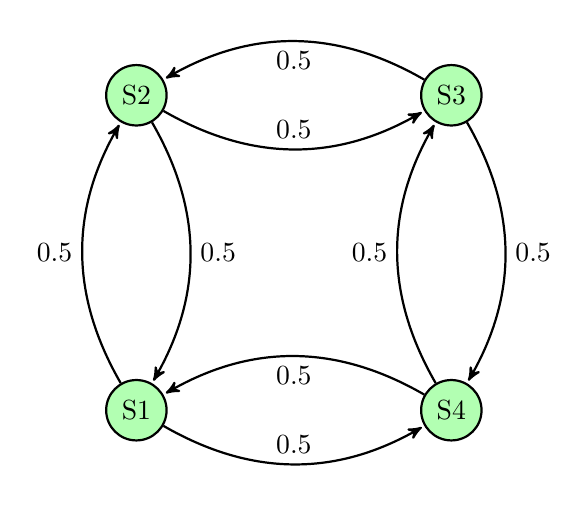
\begin{tikzpicture}[->,>=stealth',shorten >=1pt,auto,node distance=4cm,thick,main node/.style={circle,draw,font=\Large\bfseries}]
\tikzstyle{state} = [circle, draw=black, fill=green!30]
\tikzstyle{arrow} = [thick,->,>=stealth]

\node (s1) at (0,0) [state] {S1};
\node (s2) at (0,4) [state] {S2};
\node (s3) at (4,4) [state] {S3};
\node (s4) at (4,0) [state] {S4};

\path
    (s1) edge [bend right] node {0.5} (s4)
         edge [bend left] node {0.5} (s2)
    (s2) edge [bend left] node {0.5} (s1)
         edge [bend right] node {0.5} (s3)
    (s3) edge [bend right] node {0.5} (s2)
         edge [bend left] node {0.5} (s4)
    (s4) edge [bend left] node {0.5} (s3)
         edge [bend right] node {0.5} (s1);

\end{tikzpicture}
\end{center}

Once again, we can compute both myopic and non-myopic expected returns. This time, no matter the
choice of actions, there is no particular incentive for an agent to select a pair over another. If
$\rho$ is negative entropy, certain pair of actions have a higher expected return than others. But
for each $a_1$ there is a $a_2$ which obtains the maximum expected return possible.

Thus, non-myopic in this particular model has no particular advantage over a more simple myopic
solution. Once again this problem can be extended into uncountably infinite examples of Active
Perception tasks.



\bibliographystyle{unsrtnat}
\bibliography{references}

\end{document}
